\documentclass[12pt]{extarticle}

%%%% paramètres généraux
%%%% french character
\usepackage[french]{babel}
\usepackage[T1]{fontenc}
\usepackage[utf8]{inputenc}

%%%% useful packages
\usepackage[a4paper, left=1.3cm, right=1.3cm, top=2.2cm, bottom=2.3cm]{geometry}
\usepackage{subcaption} % for figure caption
\usepackage{graphicx} % image
\usepackage{tabularx} % table
\usepackage[table]{xcolor} % color in table
\usepackage{amsmath} % math
\usepackage{amssymb} % bold math
\usepackage{wasysym} % integral
\usepackage[many]{tcolorbox} % colored box
\usepackage{fancyhdr} % headers
\usepackage{enumitem} % for bullet in itemize
\usepackage[colorlinks=true,linkcolor=black,citecolor=black,filecolor=black,urlcolor=black]{hyperref} % for link
\usepackage{accents} % for complex notation
\usepackage[european, straightvoltages, RPvoltages]{circuitikz} % for electronic circuit
\usepackage{multicol} % to use several columns
\usepackage{fontawesome} % awesome icons
\usepackage{ifthen} % for loop and boolean in commands
\usepackage{pdfpages} % to include pdf
\usepackage{wrapfig} % to wrap text around figures
\usepackage{chemfig} % to draw chemistry formula
\usepackage{chemist} % surtout pour chemform
\usepackage{multirow} % for vertically merged cells
\usepackage{makecell} % to format cell in tables
\usepackage{physics} % for derivatives, braket, etc.
\usepackage{esvect} % for large vectors
\usepackage{listings} % for code
\usepackage{dashundergaps} % for automatic text to fill
% dyslexia friendly font (need to be compiled in xetex)
%\usepackage{fontspec}
%\setmainfont{OpenDyslexic}
\usepackage{tikz}
\usepackage{pgfplots}
\usepackage[framemethod=tikz]{mdframed} %pour les boîtes

%%%% settings
\setlength{\parskip}{0cm}
\setlength{\parindent}{0cm}
\renewcommand{\baselinestretch}{1}
\setcounter{tocdepth}{2}
\renewcommand{\thesection}{\textcolor{red}{\Roman{section}}}
\renewcommand{\thesubsection}{\textcolor{red}{\Roman{section}.\arabic{subsection}}}

%%%% tikz configuration
\usetikzlibrary{babel}
\tikzset{>=latex}
\usetikzlibrary{shadows}
\usetikzlibrary{backgrounds}



%%%% header
\renewcommand{\headrulewidth}{0.4pt}
\setlength{\headheight}{22.50113pt}


%%%% Table
\renewcommand{\tabularxcolumn}[1]{m{#1}}
\setlength{\extrarowheight}{8pt}


%%%% Chemfig configuration
\setchemfig{
  atom sep=20pt,
  bond style={line width=1pt},
  angle increment=30
}


%%%% dashundergaps configuration
\dashundergapssetup{
  gap-numbers = false,
  gap-format = dot,
  gap-widen,
  gap-extend-percent
}

%%%% quelques commandes
%%%%%%%%%%%%%%%%%%%%%%%%%%%%%%%%%%%%%%%%%%%%%%%%%%%%%%%%%%%%%%%%%%%%%%%%%%
%%%% quelque couleurs
\definecolor{vertSombre} {RGB}{  0,  92,  46}
\definecolor{cyanSombre} {RGB}{  0, 140, 128}
\definecolor{jauneSombre}{RGB}{138, 103,   0}
\definecolor{jauneClair} {RGB}{218, 173,   0}
\definecolor{rougeSombre}{RGB}{148,  31,   0}
\definecolor{rougeClair} {RGB}{224,  39,  34}
\definecolor{couleurtitre}{RGB}{255,  255,  255}
\definecolor{exef}{RGB}{210,210,210}
\definecolor{propositiono}{RGB}{109,109,109}

%%% quelques couleurs dérivées des couleurs choisie
\newcommand{\couleurCorrection}{couleurPrincipale!60!black}
\newcommand{\couleurExercice}{couleurPrincipale!75!black}

%%%% rectangle coloré
\newcommand\rectangle[3]{%
  \shorthandoff{;}
  \tikz \node (rect) [draw, fill, color=#1,
              minimum width=#2,
              minimum height=#3] {};
  \shorthandon{;}
}
\newcommand\rectangleCyan[2]{\rectangle{couleurPrincipale}{#1}{#2}}

%%%% simple boite
\newenvironment{boite}{
  \begin{tcolorbox}
  [ breakable, enhanced jigsaw, % to break box over page
    arc = 0mm, % straight line
    colback= white, % white background
    colframe= black % dark frame
  ]
}
{ \end{tcolorbox} }

\newtcolorbox{facile}[2][]{colback=green!5!white,
colframe=green!75!black,fonttitle=\bfseries,
colbacktitle=green!85!black,enhanced,
attach boxed title to top center={yshift=-2mm},
title={#2},#1}

\newtcolorbox{difficile}[2][]{colback=red!5!white,
colframe=red!75!black,fonttitle=\bfseries,
colbacktitle=red!85!black,enhanced,
attach boxed title to top center={yshift=-2mm},
title={#2},#1}


%\newenvironment[1]{Propriete}{\begin{tcolorbox}[colback=red!5!white,colframe=red!75!black,title=\textbf{#1 :}]
%}
%{\end{tcolorbox} 


%%%%%%%%%%%%%%%%%%%%%%%%%%%%%%%%%%%%%%%%%%%%%%%%%%%%%%%%%%%%%%%%%%%%%%%%%%
%%%% pagination et sections
\newcommand{\titre}[1]{
  \begin{center}
    \textsf{\bfseries \Large #1}
  \end{center}
}
\newcommand{\sousTitre}[1]{
  \textsf{\bfseries #1}
}
\newcommand{\pasDePagination}{
  \thispagestyle{empty}
}
\newcommand{\feuilleBlanche}{
  \newpage
  \phantom{b}
  \pasDePagination
}


%%%% activité ou TP
\newcounter{acti}
\newcommand{\titreActi}[2]{
  \refstepcounter{acti}
  \titre{#1 \arabic{section}.\arabic{acti} -- #2}
}
\newcommand{\titreTP}[1]{
  \titreActi{TP}{#1}
  %\titreActi{Activité expérimentale}{#1}
}
\newcommand{\titreActivite}[1]{
  \titreActi{Activité}{#1}
}
\newcommand{\titreEvaluation}[1]{
  \titreActi{Évaluation}{#1}
}


%%%% chapitre, section et sous-section
\newcommand{\titreChapitre}[1]{
  \titre{Chapitre \arabic{section} : #1}
}
\newcommand{\titrePartie}[1]{
  \vspace*{24pt}
  \refstepcounter{subsection}
  \rectangleCyan{60pt}{1pt}
  \sousTitre{\Large \Roman{subsection} -- #1}
  \rectangleCyan{60pt}{1pt}
  \vspace*{10pt}
}
\newcounter{sousSection}
\newcommand{\titreSection}[1]{
  \vspace*{16pt}
  \refstepcounter{subsubsection}
  \setcounter{sousSection}{0}
  \rectangleCyan{30pt}{4pt}
  \sousTitre{\large \arabic{subsubsection} -- #1}
  \vspace*{10pt}
}
\newcommand{\titreSousSection}[1]{
  \vspace*{12pt}
  \refstepcounter{sousSection}
  \sousTitre{\Alph{sousSection} -- #1}
  \vspace*{8pt}
}

%%%% fixe le numéro de l'activité
\newcommand{\numeroActivite}[1]{
  \setcounter{subsection}{0}
  \setcounter{subsubsection}{0}
  \setcounter{sousSection}{0}
  \setcounter{figure}{0}
  \setcounter{document}{0}
  \setcounter{exercice}{0}
  \setcounter{QCM}{0}
  \setcounter{countCoupDePouce}{0}
  \setcounter{acti}{#1 - 1}
  \setcounter{page}{1}
}
% fixe le numéro de page (#2) et de partie (#1)
\newcommand{\numeroPartieCours}[2]{
  \newpage
  \setcounter{subsection}{#1 - 1}
  \setcounter{page}{#2}
}

%%%% lignes
\newcommand{\ligne}{
  \par\noindent\rule{\textwidth}{0.4pt}
}
\newcommand{\lignePointillee}[1]{
  \makebox[#1\textwidth]{\dotfill}
}


%%%%%%%%%%%%%%%%%%%%%%%%%%%%%%%%%%%%%%%%%%%%%%%%%%%%%%%%%%%%%%%%%%%%%%%%%%
%%%% en-tête
\newcommand{\teteGauche}[1]{
  \lhead{
    \textbf{\footnotesize #1}
  }
}
\newcommand{\teteDroite}[1]{
  \rhead{
    \hfill \textbf{\footnotesize #1}
  }
}

%

\newcommand{\enTeteRevision}[2]{
  \pagestyle{fancy}
  \lhead{Revision #1 - \textit{#2}}
  %\chead{} % central header
  \teteDroite{Lycée Parc de Vilgénis 2023 - 2024}
}

\newcommand{\enTeteMethodo}[2]{
  \pagestyle{fancy}
  \teteGauche{Fiche Méthode #1 : #2}
  %\chead{} % central header
  \teteDroite{Lycée Parc de Vilgénis 2023 - 2024}
}

\newcommand{\enTeteChap}[2]{
  \pagestyle{fancy}
  \lhead{Chapitre #1 - \textit{#2}}
  %\chead{} % central header
  \teteDroite{Lycée Parc de Vilgénis 2023 - 2024}
}

\newcommand{\enTeteExo}[1]{
  \pagestyle{fancy}
  \lhead{Exercices du Chapitre #1}
  %\chead{} % central header
  \teteDroite{Lycée Parc de Vilgénis 2023 - 2024}
}

\newcommand{\enTeteAct}[3]{
  \pagestyle{fancy}
  \lhead{Chapitre #1 \newline Activité #2 - \textit{#3}}
  %\chead{} % central header
  \teteDroite{Lycée Parc de Vilgénis 2023 - 2024}
}

\newcommand{\enTeteDM}[2]{
  \pagestyle{fancy}
  \lhead{Devoir Maison n$\degree$ #1 - \textit{#2}}
  %\chead{} % central header
  \teteDroite{Lycée Parc de Vilgénis 2023 - 2024}
}

\newcommand{\enTeteTP}[2]{
  \pagestyle{fancy}
  \lhead{TP #1 - \textit{#2}}
  %\chead{} % central header
  \teteDroite{Lycée Parc de Vilgénis 2023 - 2024}
}
%
\newcommand{\enTeteSeance}[2]{
  \pagestyle{fancy}
  \lhead{Date : \textit{#1}}
  \chead{Séance : #2}
  \teteDroite{Seconde} % central header
}
%

\newcommand{\enTeteFicheReussite}[1]{
  \newpage
  \setcounter{subsection}{0}
  \pasDePagination
  
  \phantom{b}
  \vspace*{-70pt}
  \titre{Fiche \og Réussir son évaluation \fg}
  \titre{#1}
  
  \vspace*{-6pt}
  % \titreSection{Ce que je dois savoir}
  
  Pour savoir quoi réviser, je lis les points clés du chapitre évalués :
  \begin{itemize}
    \item Si je pense maîtriser une notion, je coche la case \ok
    \item Si je pense que je dois la retravailler, je coche la case \pasOk
  \end{itemize}
  
  Pour travailler les notions qui ne sont pas maîtrisées, je reprend les activités associés.
}
\newcommand{\basDePageFicheReussite}{
  \titreSection{Ce qu'il me reste à faire}
}
\newcommand{\travailExerciceCorrige}{
  Pour être sûr-e d'obtenir une bonne note, je m'entraîne avec les exercices corrigés du manuel indiqués dans la colonne de droite.
}
\newcommand{\questionFicheReussite}[1]{
  S'il me reste des questions, je les note ici pour les poser au début de l'évaluation :\\[4pt]
  \lignesReponse{#1}
}
\newcommand{\coursFicheReussite}{
  Je prépare une fiche au format A4 avec toutes les notions, définitions ou grandeurs dont je pense avoir besoin pendant l'évaluation.
}


%%%%%%%%%%%%%%%%%%%%%%%%%%%%%%%%%%%%%%%%%%%%%%%%%%%%%%%%%%%%%%%%%%%%%%%%%%
%%%% exercice
% définit un booléen pour entrer ou sortir du mode correction
\newboolean{modeProf}
\setboolean{modeProf}{false}
\newcommand{\modeCorrection}{
  \setboolean{modeProf}{true}
  \TeacherModeOn
}

% définit une commande pour afficher une question 
% #1 : question
% #2 : réponse
% #3 : nombres de lignes pour répondre
\newcommand{\question}[3]{
  \numeroQuestion\!#1
  
  % pointille ou correction
  \ifthenelse {\boolean{modeProf}} { % prof
    \reponseCorrigee{#2}
  }{ % eleve
    \vspace*{8pt}
    \lignesReponse{#3}
  }
}

%
\newcounter{exercice}
\newcommand{\numeroQuestion}{
  \refstepcounter{exercice}
  \vspace*{2pt}
  \hspace{15pt}
  \textcolor{black}{%couleurPrincipale!75!black}{
    \textbf{\arabic{exercice}} {\small\faMinus}
  }
}

% correction
\newcommand{\reponseCorrigee}[1]{
  \vspace*{2pt}
  \hspace{16pt}
  \textcolor{red}{
    \faCaretRight \hspace{2pt} #1
  }
}
\newcommand{\correction}[1]{
  \ifthenelse {\boolean{modeProf}} { % prof
    \textcolor{red}{#1}
  }{ % eleve
  }
}

% trace des lignes pour répondre
\newcounter{int}
\newcommand{\lignesReponse}[1]{
  \setcounter{int}{-1}
  \loop
    \stepcounter{int}
    \ifnum \value{int} < #1
    \lignePointillee{0.99} \\[8pt]
  \repeat
  \ifnum #1 > 0
    \vspace*{-12pt}
  \fi
}

% sous questions
\newcommand{\sousQuestion}[2]{
  \hspace{15pt}
  \textcolor{couleurPrincipale!75!black}{\textbullet} #1
  
  \vspace*{8pt}
  \reponse{#2}
}


%%%%%%%%%%%%%%%%%%%%%%%%%%%%%%%%%%%%%%%%%%%%%%%%%%%%%%%%%%%%%%%%%%%%%%%%%%
%%%% QCM
% question QCM
\newcounter{QCM}
\newcommand{\QCM}[2]{
  \refstepcounter{QCM}
  \vspace*{2pt}
  \textcolor{couleurPrincipale!75!black}{\textbf{\arabic{QCM}} {\small\faMinus}} #1
  
  \begin{qcm}
    #2
  \end{qcm}
}


%%%% Pour afficher les compétences
\newcommand{\competence}[1]{
  ~{\footnotesize\textit{(#1)}}
}


%%%% Espace pour indiquer nom, prénom et classe
\newcommand{\nomPrenomClasse}{
  \vspace*{-24pt}
  \underline{Nom} : \lignePointillee{0.3}\hfill \underline{Date } : \gap{....}/\gap{....}/\gap{....} \newline 
  \underline{Prénom} : \lignePointillee{0.3} \hfill\underline{Classe} : \gap{........}
}


%%%%%%%%%%%%%%%%%%%%%%%%%%%%%%%%%%%%%%%%%%%%%%%%%%%%%%%%%%%%%%%%%%%%%%%%%%
% texte à trou automatique
\newcommand{\texteTrouAuto}[1]{
  \gap{
    \textcolor{couleurPrincipale!60!black}{ \textbf{#1} }
  }
}

% texte à trou dans une ligne réglable
\newcommand{\texteTrou}[2]{
  \ifthenelse {\boolean{modeProf}} {% prof
    \textcolor{couleurPrincipale!60!black}{ \textbf{#1} }
  }{% élève
    \espaceReponse
    \lignePointillee{#2}
  }
}

% texte à trou sur plusieurs lignes
\newcommand{\texteTrouLigneComplete}[1]{
  \ifthenelse {\boolean{modeProf}} {% prof
    \textcolor{couleurPrincipale!60!black}{ \textbf{#1} }
  }{% élève
    \espaceReponse \dotfill
  }
}

% texte à trou sur plusieurs lignes
\newcommand{\texteTrouMultiLignes}[2]{
  \ifthenelse {\boolean{modeProf}} {% prof
    \textcolor{couleurPrincipale!60!black}{ \textbf{#1} }
  }{% élève
    \reponseLigne
    \lignesReponse{#2}
  }
}

% reponse en fin de ligne
\newcommand{\reponseLigne}{
  \espaceReponse
  \dotfill \\[8pt]
}

% espace vertical pour la réponse
\newcommand{\espaceReponse}{
  \phantom{$\Frac{1}{1}$} % espace vertical
  \hspace*{-40pt} \phantom{b} % ajuste l'espace horizontal
}

%%%%%%%%%%%%%%%%%%%%%%%%%%%%%%%%%%%%%%%%%%%%%%%%%%%%%%%%%%%%%%%%%%%%%%%%%%
%%%% Pour choisir parmi deux sujets
\newboolean{sujetA}
\setboolean{sujetA}{true}
\newcommand{\sujetB}{
  \setboolean{sujetA}{false}
}
\newcommand{\sujetA}{
  \setboolean{sujetA}{true}
}

%%%% Pour faire plusieurs sujets en parallèle
\newcommand{\variationSujet}[2]{
  \ifthenelse {\boolean{sujetA}}
  {\hspace*{-2pt}#1\hspace*{-2pt}}
  {\hspace*{-2pt}#2\hspace*{-2pt}}
}


%%%%%%%%%%%%%%%%%%%%%%%%%%%%%%%%%%%%%%%%%%%%%%%%%%%%%%%%%%%%%%%%%%%%%%%%%%
%%%% documents
\newcounter{document}
\newcommand{\titreDocu}[1]{
  \refstepcounter{document} % update counter
  \textbf{Document \arabic{document} -- #1} % print document title
  \addcontentsline{toc}{document}{\protect\numberline{} #1} % update table of content
}
\newenvironment{doc}[1]{
  \begin{boite}
    \titreDocu {#1} \newline
}
{ \end{boite} }

%\newenvironment{exo}[1]{
%\begin{mdframed}[style=autreexo]
%\textbf{\bsc{Exercice de cours 1} - Espèces chimiques}\\
%Donner le type (\textit{atomique}, \textit{moléculaire} ou \textit{ionique}) des espèces chimiques suivantes : hélium (He), eau (H\textsubscript{2}O), chlorure de sodium (Na$^{+}$, Cl$^{-}$).
%\end{mdframed}
%}
%% pour les référencer
\newcommand{\docu}[1]{
  \textbf{(Doc. #1)}
}


%%%% problematique
\newcommand{\problematique}[1]{
  %\hspace{8pt}
  \noindent\textcolor{red}{\begin{large} \textbf{\underline{Problématique} : }\end{large}}\textbf{#1}
  }



%%%% objectifs
\newenvironment{objBoite}{
  \begin{tcolorbox}
  [boxrule = 0pt,
  frame hidden, sharp corners,
  colback = white, enhanced,
  borderline north={2pt}{0pt}{couleurPrincipale},
  borderline south={2pt}{0pt}{couleurPrincipale},
  borderline west={4pt}{0pt}{couleurPrincipale},
  borderline east={4pt}{0pt}{couleurPrincipale}
  ]
  
}
{
  \end{tcolorbox}
}
\newenvironment{objectifs}{
  \begin{objBoite}
    \begin{center}
      \sousTitre{\large Objectifs de la séance :}
      \begin{listeObjectifs}
}
{ 
      \end{listeObjectifs}
    \end{center}
  \end{objBoite}
}

%%%% Espace pour un coup de pouce
\newcounter{countCoupDePouce}
\newenvironment{coupDePouce}{
  \refstepcounter{countCoupDePouce}
  \vspace*{-12pt}
  \begin{boite}
    \begin{flushright}
      \textcolor{couleurPrincipale}{\faSquareO}
    \end{flushright}
    
    \vspace*{-30pt}
    \textcolor{couleurPrincipale}{\faThumbsUp}
    \textbf{Coup de pouce \arabic{countCoupDePouce}} :\\[4pt]
}
{
  \end{boite}
}


%%%% Espace pour une appréciation
\newcommand{\appreciation}[1]{
  \vspace*{8pt}
  \sousTitre{Appréciation et remarques}
  \vspace*{-8pt}
  \begin{boite}
    \vspace{#1 pt}
    \phantom{b}
  \end{boite}
}


%%%%%%%%%%%%%%%%%%%%%%%%%%%%%%%%%%%%%%%%%%%%%%%%%%%%%%%%%%%%%%%%%%%%%%%%%%
%%%% Définit un nouveau type de colonne : taille fixée par une fraction
%%%% de la largeur de la ligne, avec un texte centré
\newcolumntype{C}[1]{>{\centering\arraybackslash}p{#1\linewidth}}

%%%% Tableau de competence
\newenvironment{tableauCompetences}{
  \centering
  \setlength{\extrarowheight}{6pt}
  \tabularx{\linewidth}{| c | X | c | c | c | c |}
    \hline
    \rowcolor{blue!25}
    \centering \textbf{Compétences} & \centering \textbf{Items} & \textbf{D} & \textbf{C} & \textbf{B} & \textbf{A}
    \\ \hline
}
{
    \\ \hline
  \endtabularx
}

%%%% Tableau de connaissances
\newenvironment{tableauConnaissances}{
  \centering
  \setlength{\extrarowheight}{6pt}
  \tabularx{\linewidth}{| X | c | c | C{0.18} | C{0.15} |}
    \hline
    \rowcolor{gray!20} 
    \textbf{Points clés du chapitre} & \ok & \pasOk & \textbf{En classe} & \textbf{Exercices}
    \\ \hline
}
{   
    \\ \hline
  \endtabularx
}

%%%% Tableau de connaissances sans exercices
\newenvironment{tableauConnaissancesSansExercices}{
  \centering
  \setlength{\extrarowheight}{6pt}
  \tabularx{\linewidth}{| X | c | c | C{0.2} |}
    \hline
    \rowcolor{gray!20} 
    \textbf{Points clés du chapitre} & \ok & \pasOk & \textbf{En classe}
    \\ \hline
}
{   
    \\ \hline
  \endtabularx
}

%%%% Tableau de correction élève
\newcommand{\correctionEleve}[1]{
  \setlength{\extrarowheight}{6pt}
  \begin{tabularx}{\linewidth}{| X | C{0.26} | C{0.26} | C{0.26} |}
    \hline
    \rowcolor{gray!20}
    \textbf{Question} &
    \textbf{L'erreur} &
    \textbf{Analyse de l'erreur} &
    \textbf{La correction}
    \\ \hline
    %
    \phantom{b} \vspace{#1 pt}
    & & & \\ \hline
    \phantom{b} \vspace{#1 pt}
    & & & \\ \hline
    \phantom{b} \vspace{#1 pt}
    & & & \\ \hline
    \phantom{b} \vspace{#1 pt}
    & & & \\ \hline
  \end{tabularx}
}

%%%% Tableau bilan de la correction
\newcommand{\bilanCorrection}[1]{
  \setlength{\extrarowheight}{6pt}
  \begin{tabularx}{\linewidth}{| X | X |}
    \hline
    \rowcolor{gray!20}
    \textbf{Ce que je n'avais pas compris...} &
    \textbf{Ce que maintenant j'ai compris...}
    \\ \hline
    \phantom{b} \vspace{#1 pt} % \newline \newline \newline
    & \\ \hline
  \end{tabularx}
}


%%%%%%%%%%%%%%%%%%%%%%%%%%%%%%%%%%%%%%%%%%%%%%%%%%%%%%%%%%%%%%%%%%%%%%%%%%
%%%% symboles : chevron, flèche, attention, etc.
\newcommand{\chevron}{
  \textcolor{couleurPrincipale}{\small \faChevronRight}
}
%
\newcommand{\fleche}{
  \textcolor{couleurPrincipale}{\faCaretRight}
}
%
\newcommand{\attention}{
  \textcolor{couleurPrincipale}{\faExclamationTriangle}
}
%
\newcommand{\flecheLongue}{
  \textcolor{red}{\longrightarrow}
}
%
\newcommand{\ok}{
  \textcolor{couleurPrincipale}{\faCheckCircle}
}
%
\newcommand{\pasOk}{
  \textcolor{couleurPrincipale}{\faTimesCircle}
}
%
\newcommand{\pointCyan}{
  \textcolor{couleurPrincipale}{\textbullet}
}
%
\newcommand{\mesure}{
  \hspace{15pt}
  \textcolor{couleurPrincipale!75!black}{\faWrench\faFlask}
}


%%%%%%%%%%%%%%%%%%%%%%%%%%%%%%%%%%%%%%%%%%%%%%%%%%%%%%%%%%%%%%%%%%%%%%%%%%
%%%% Passage important
\newenvironment{definition}[1]{
  \begin{tcolorbox}[colback=green!5!white,colframe=green!75!black,title=\textbf{#1}]
  
}
{
  \end{tcolorbox}
}

%%%% contexte
\newenvironment{contexte}{
  \begin{tcolorbox}
  [boxrule = 4pt, sharp corners,
  colframe = couleurPrincipale,
  colback = white!95!couleurPrincipale, % background color
  breakable, enhanced jigsaw] % to break box over page
  
}
{
  \end{tcolorbox}
}


%%%% emphase
\newcommand{\emphase}[1]{
  \textcolor{couleurImportant}{\textsf{\bfseries \large #1}}
}
%
\newcommand{\important}[1]{
  \!\textcolor{green}{\textbf{\bfseries #1}}\!\!
}
%
\newcommand{\exemple}{
  \flecheLongue \textit{Exemple :}
}
\newcommand{\exemples}{
  \flecheLongue \textit{Exemples :}
}
%
\newcommand{\note}{
  \textbf{Note :}
}
%
\newcounter{appelProf}
\newcommand{\appelProf}{
  \refstepcounter{appelProf}
  \hspace{24pt} \faHandPaperO \hspace{2pt}
  \textbf{Appel n$^\circ$ \arabic{appelProf} :}
}


%%%% image
\newcommand{\image}[2]{
  \includegraphics[width=#1\linewidth]{#2}
}


%%%%%%%%%%%%%%%%%%%%%%%%%%%%%%%%%%%%%%%%%%%%%%%%%%%%%%%%%%%%%%%%%%%%%%%%%%
%%%% qcm
\newlist{qcm}{itemize}{2}
\setlist[qcm]{label=$\square$, leftmargin=2cm}


%%%% liste d'objectif
\newlist{listeObjectifs}{itemize}{2}
\setlist[listeObjectifs]{label = \chevron}


%%%% protocole
\newlist{protocole}{itemize}{2}
\setlist[protocole]{label = {\footnotesize \fleche}}


%%%% liste de points
\newlist{listePoints}{itemize}{2}
\setlist[listePoints]{label = \pointCyan}


%%%% jeu de données
\newenvironment{donnees}{
  \textbf{Données :}
  \begin{listePoints}
}{
  \end{listePoints}
}


%%%% liste avec chiffre
\newlist{enumeration}{enumerate}{2}
\setlist[enumeration]{label = \textcolor{couleurPrincipale!75!black}{\textbf{\arabic*.}} }


%%%%%%%%%%%%%%%%%%%%%%%%%%%%%%%%%%%%%%%%%%%%%%%%%%%%%%%%%%%%%%%%%%%%%%%%%%
%%%% Séparation de la page
\newcommand{\separationTroisBlocs}[3]{
  \begin{minipage}[t]{0.3\linewidth}
    #1
  \end{minipage}
  ~
  \begin{minipage}[t]{0.3\linewidth}
    #2
  \end{minipage}
  ~
  \begin{minipage}[t]{0.3\linewidth}
    #3
  \end{minipage}
}
%%%%
\newcommand{\separationDeuxBlocs}[2]{
  \begin{minipage}[t]{0.48\linewidth}
    #1
  \end{minipage}
  \hfill
  \begin{minipage}[t]{0.48\linewidth}
    #2
  \end{minipage}
}
\newcommand{\separationBlocs}[4]{
  \begin{minipage}[t]{#1\linewidth}
    #3
  \end{minipage}
  \hfill
  \begin{minipage}[t]{#2\linewidth}
    #4
  \end{minipage}
}


%%%%%%%%%%%%%%%%%%%%%%%%%%%%%%%%%%%%%%%%%%%%%%%%%%%%%%%%%%%%%
%%%% tikz macros
%%%% rectangle
\newcommand{\tkzRect}[4]{
  \fill[color=#1] (#2,#4) -- (-#2,#4) -- (-#2,#3) -- (#2,#3);
}
\newcommand{\tkzEllipse}[4]{
  \fill[color=#1] (0,#3) ellipse (#2 and #4);
}
\newcommand{\tkzLegende}[4]{
  \draw[black, ->, very thick] (#2 + #4, #3) node[right] {#1} -- (#2, #3);
}
\newcommand{\tkzCercle}[4]{
  \filldraw [#3] (#1, #2) circle (#4pt);
}
\newcommand{\tkzCercleLigne}[5]{
  \filldraw [color = #4, fill = #3, very thick] (#1, #2) circle (#5pt);
}
%%%% tube à essais
\newcommand{\tkzTubeEssai}[3]{
  \draw[thick] (#1,#2) -- (#1,0) arc (0:-180:#1) -- (-#1,#2);
  \draw[thick] (0,#2) ellipse (#1 and #3);
}
\newcommand{\tkzBasTubeEssai}[5]{
  \fill[color=#1] (-#2,#3) -- (#2,#3) arc (0:-180:#2);
  \tkzRect{#1}{#2}{#3 - 0.01}{#4}
  \tkzEllipse{#1!85!black}{#2}{#4}{#5}
}
\newcommand{\tkzPhaseTubeEssai}[5]{
  \tkzRect{#1}{#2}{#3}{#4}
  \tkzEllipse{#1}{#2}{#3}{#5}
  \tkzEllipse{#1!85!black}{#2}{#4}{#5}
}

%%%% Point et vecteurs
\newcommand{\tkzLabel}[3]{
  \node at (#1, #2) {#3};
}
\newcommand{\tkzPointLabel}[3]{
  \filldraw (#1, #2) circle (2pt) node[above] {#3};
}
\newcommand{\tkzVecteur}[6]{
  \draw[black, ->, very thick] (#1, #2) -- (#1 + #3, #2 + #4) node[#6] {#5};
}
\newcommand{\tkzEquiv}[6]{
  \draw[black, <->, thick] (#1, #2) -- (#1 + #3, #2 + #4);
  \draw[black] (#1 + #3/2, #2 + #4/2) node[#6] {#5};
}
\newcommand{\tkzVecteurX}[4]{
  \draw[black, ->, very thick] (#1, #2) -- (#1 + #3, #2) node[above] {#4};
}
\newcommand{\tkzVecteurY}[4]{
  \draw[black, ->, very thick] (#1, #2) -- (#1, #2 + #3) node[right] {#4};
}
\newcommand{\tkzEquivY}[5]{
  \draw[#1, <->, thick] (#2, #3) -- (#2, #3 + #4);
  \draw[#1] (#2, #3 + #4/2) node[right] {#5};
}
\newcommand{\tkzEquivX}[5]{
  \draw[#1, <->, thick] (#2, #3) -- (#2 + #4, #3);
  \draw[#1] (#2 + #4/2, #3) node[below] {#5};
}

%%%% plan de classe
\newcommand{\rectangleTexte}[5]{
  \filldraw [fill=white, draw=black, ultra thick] (#1, #2) rectangle (#1 + #3, #2 + #4);
  \node at (#1 + #3/2, #2 + #4/2) [font=\sffamily] {\textbf{\large #5}};
}
% place dans la classe
\newcommand{\place}[3]{
  \rectangleTexte{#1}{#2}{3}{2}{#3}
}
\newcommand{\deuxPlaces}[4]{
  \place{#1}{#2}{#3}
  \place{#1 + 3}{#2}{#4}
}
\newcommand{\troisPlaces}[5]{
  \place{#1}{#2}{#3}
  \place{#1 + 3}{#2}{#4}
  \place{#1 + 6}{#2}{#5}
}
\newcommand{\quatrePlaces}[6]{
  \place{#1}{#2}{#3}
  \place{#1 + 3}{#2}{#4}
  \place{#1 + 6}{#2}{#5}
  \place{#1 + 9}{#2}{#6}
}
%%%% rangée
\newboolean{quatrePlace}
\setboolean{quatrePlace}{false}
\newcommand{\avecQuatrePlaces}{ \setboolean{quatrePlace}{true} }
\newcommand{\avecTroisPlaces}{ \setboolean{quatrePlace}{false} }
\newcommand{\rangee}[9]{
  \ifthenelse {\boolean{quatrePlace}} {
    \deuxPlaces  {0}{#1} {#2}{#3}
    \quatrePlaces{7}{#1} {#4}{#5}{#6}{#7}
    \deuxPlaces  {20}{#1}{#8}{#9}
  }{
    \deuxPlaces {#1}{#2}     {#3}{#4}
    \troisPlaces{#1 + 7}{#2} {#5}{#6}{#7}
    \deuxPlaces {#1 + 17}{#2}{#8}{#9}
  }
}
\newcommand{\rang}[9]{
  \ifthenelse {\boolean{quatrePlace}} {
    \deuxPlaces  {0} {12 - 3*#1} {#2}{#3}
    \quatrePlaces{7} {12 - 3*#1} {#4}{#5}{#6}{#7}
    \deuxPlaces  {20}{12 - 3*#1} {#8}{#9}
  }{
    \deuxPlaces {0} {12 - 3*#1} {#2}{#3}
    \troisPlaces{7} {12 - 3*#1} {#4}{#5}{#6}
    \deuxPlaces {17}{12 - 3*#1} {#7}{#8}
  }
}

%%%% TP
\newcommand{\paillasse}[3]{
  \rectangleTexte{#1}{#2}{4}{2}{#3}
}
\newcommand{\rangeeTP}[6]{
  \paillasse{#1}{#2}     {#3}
  \paillasse{#1 + 4}{#2} {#4}
  \paillasse{#1 + 12}{#2}{#5}
  \paillasse{#1 + 16}{#2}{#6}
}


%%%%%%%%%%%%%%%%%%%%%%%%%%%%%%%%%%%%%%%%%%%%%%%%%%%%%%%%%%%%%%%%%%%%%%%%%%
%%%% unité, degré, vecteur, etc.
\newcommand{\unit}[1]{
  \; \mathrm{#1}
}
\newcommand{\unitb}[1]{
  \unit{\mathbf{#1}}
}
\newcommand{\degree}{
  ^\circ\!
}
\newcommand{\degreCelsius}{
  \degree\, \mathrm{C}
}
\newcommand{\Frac}[2]{
  \displaystyle \frac{#1}{#2}
}
\newcommand{\algebrique}[1]{
  \overline{\mathrm{#1}}
}
\newcommand{\reaction}{
  \!\!\schemestart \arrow(.mid east--.mid west){->}[, 0.9, ultra thick] \schemestop\!\!
}
\newcommand{\metreParSeconde}{
  \unit{m\cdot s}^{-1}
}
%% grandeurs
\newcommand{\gISS}{g_\text{ISS}}
\newcommand{\MTerre}{M_\text{Terre}}
\newcommand{\RTerre}{R_\text{Terre}}
\newcommand{\inertie}{\text{inertie}}
\newcommand{\Tfus}{ T_{\text{f}} }
\newcommand{\Teb}{ T_{\text{éb}} }
\newcommand{\avogadro}{6,\!02 \times 10^{23}}
\newcommand{\saccha}{Saccharose (\chemfig{C_{12} H_{22} O_{11}})}
\newcommand{\vitamC}{Vitamine C (\chemfig{C_{6} H_{8} O_{6}})}
\newcommand{\ionsCa}{Ion calcium (\chemfig{Ca^{2+}})}
%% vecteurs
\newcommand{\FBsurA}{
  F_{B/A}
}
\newcommand{\FAsurB}{
  F_{A/B}
}
\newcommand{\vvFAsurB}{
  \vv{F}_{A/B}
}
\newcommand{\vvFBsurA}{
  \vv{F}_{B/A}
}

%% atome et isotope
\makeatletter
\newcommand{\isotope}[3]{%
   \settowidth\@tempdimb{\ensuremath{\scriptstyle#1}}%
   \settowidth\@tempdimc{\ensuremath{\scriptstyle#2}}%
   \ifnum\@tempdimb>\@tempdimc%
       \setlength{\@tempdima}{\@tempdimb}%
   \else%
       \setlength{\@tempdima}{\@tempdimc}%
   \fi%
  \begingroup%
  \ensuremath{
    ^{\makebox[\@tempdima][r]{\ensuremath{\scriptstyle#1}}}
    _{\makebox[\@tempdima][r]{\ensuremath{\scriptstyle#2}}}
    \chemfig{#3}
  }%
  \endgroup%
}%
\makeatother
%% element chimique
\makeatletter
\newcommand{\element}[2]{%
   \settowidth\@tempdimb{\ensuremath{\footnotesize #1}}%
  \begingroup%
  \ensuremath{
    _{\makebox[\@tempdimb][r]{\ensuremath{\small #1}}} 
    \chemfig[atom style={scale=1.3}]{#2}
  }%
  \endgroup%
}%
\makeatother

%% siècle
\newcommand{\siecle}[1]{
  \textsc{\romannumeral #1}\textsuperscript{e}~siècle
}
%% texte avec une boite autour
\newcommand{\texteEncadre}[1]{
  \frame{\vphantom{$\Frac{1}{10}$} \text{ #1 } }
}


%% papier millimétré
\newcommand{\papiermillimetre}{
\begin{tikzpicture}
	% Dimensions du repere
	\def\xmin{0} \def\xmax{18} \def\ymin{0} \def\ymax{25}
	% Grilles
	\draw [step=0.1cm,gray,ultra thin]  (\xmin,\ymin) grid (\xmax,\ymax);
	\draw [step=0.5cm,gray, thin] (\xmin,\ymin) grid (\xmax,\ymax);
	\draw [step=1cm,gray, thick] (\xmin,\ymin) grid (\xmax,\ymax);
	\draw [step=5cm,gray,very thick] (\xmin,\ymin) grid (\xmax,\ymax);
\end{tikzpicture}
}


%%%%%%%%%%%%%%%%%%%%%%%%%%%%%%%%%%%%%%%%%%%%%%%%%%%%%%%%%%%%%%%%%%%%%%%%%%
%%%% Couleur pour le code
\definecolor{vertCode}    {rgb}{0.2,0.6,0}
\definecolor{grisCode}    {rgb}{0.5,0.5,0.5}
\definecolor{violetCode}  {rgb}{0.58,0,0.82}
\definecolor{fondCode}    {rgb}{0.95,0.95,0.92}
%%%% Style python
\lstdefinestyle{codePython}{
    backgroundcolor=\color{fondCode},
    commentstyle=\color{magenta},
    keywordstyle=\color{vertCode},
    numberstyle=\tiny\color{grisCode},
    stringstyle=\color{violetCode},
    basicstyle=\ttfamily\footnotesize,
    breakatwhitespace=false,
    breaklines=true,
    captionpos=b,
    keepspaces=true,
    numbers=left,
    numbersep=5pt, 
    showspaces=false,
    showstringspaces=false,
    showtabs=false, 
    tabsize=2
}
\def\inline{\lstinline[style=codePython,language=python]}


%%%% Commande pour les boîtes (def, titre, ...)

\global\mdfdefinestyle{titr}{backgroundcolor=couleurtitre, shadow=false, linewidth=1pt, linecolor=red, shadowsize=5pt}

\global\mdfdefinestyle{autreexo}{backgroundcolor=exef, shadow=false, linewidth=2pt, linecolor=propositiono, topline=false, rightline=false, bottomline=false}


%%%%%%%%%%%%%%%%%%%%%%%%%%%%%%%%%%%%%%%%%%%%%%%%%%%%%%%%%%%%%%%%%%%%%%%%%%
%%%% Chapitres
\newcommand{\sndChapitreUn}{\textbf{Fiche Méthode 1}}
\newcommand{\sndChapitreDeux}  {Mouvement et interactions}
\newcommand{\sndChapitreTrois} {Atomes et molécules}
\newcommand{\sndChapitreQuatre}{Ondes lumineuses et optique}
\newcommand{\sndChapitreCinq}  {Transformations de la matière et réactions nucléaires}
\newcommand{\sndChapitreSix}   {Réactions chimiques}
\newcommand{\sndChapitreSept}  {Signaux et capteurs}
\newcommand{\sndChapitreHuit}  {Ondes sonores}

%%%% Révisions
\newcommand{\sndRevision}{Révisions}

%%%% en-tête
\newcommand{\sndEnTeteRevision}{\newpage \enTeteRevision{1}{Exercices de révisions du collège}}
%
\newcommand{\sndEnTeteTPO}{\newpage \enTeteTP{0}{Des mesures en tout sens}}
%
\newcommand{\sndEnTeteTPUn}{\newpage \enTeteTP{1}{Identification des espèces chimiques}}
%
\newcommand{\sndEnTeteTPDeux}{\newpage \enTeteTP{2}{Mais qui a pollué la Seine ?}}
%
\newcommand{\sndEnTeteMethodoUn}  {\newpage \enTeteMethodo{1}}
%
\newcommand{\sndEnTeteCoursUn}   {\newpage \enTeteChap{1}{Corps purs et mélanges au quotidien}}
%
\newcommand{\sndEnTeteActUn}   {\newpage \enTeteAct{1}{1}{Composition d'un mélange}}
%
\newcommand{\sndEnTeteDMUn}   {\newpage \enTeteDM{1}{Composition de l'air}}
%%%%%%%%%%%%%%%%%%%%%%%%%%%%%%%%%%%%%%%%%%%%%%%%%%%%
\newcommand{\sndEnTeteActDeux}   {\newpage \enTeteAct{2}{1}{Concentration en masse}}
%
\newcommand{\seanceUn}{\newpage \enTeteSeance{07/09/2023}{Présentation de rentrée}}
%
\newcommand{\sndEnTeteTPTrois}{\newpage \enTeteTP{3}{Composition d'un alcool pharmaceutique}}
%
\newcommand{\sndEnTeteTPQuatre}{\newpage \enTeteTP{4}{Dosage d'une solution anticeptique}}
%
\newcommand{\sndEnTeteCoursDeux}   {\newpage \enTeteChap{2}{Les solutions acqueuses}}
%
\newcommand{\sndEnTeteExerciceDeux} {\newpage \enTeteExo{2}}
\newcommand{\sndEnTeteQuatre}{\newpage \enTete{\sndChapitreQuatre}{4}}
\newcommand{\sndEnTeteCinq}  {\newpage \enTete{\sndChapitreCinq}{5}}
\newcommand{\sndEnTeteSix}   {\newpage \enTete{\sndChapitreSix}{6}}
\newcommand{\sndEnTeteSept}  {\newpage \enTete{\sndChapitreSept}{7}}
\newcommand{\sndEnTeteHuit}  {\newpage \enTete{\sndChapitreHuit}{8}}



%\fancyhead[L]{\textit{\textcolor{blue!20!red}{\textbf{Cours Chimie}} - Seconde}}
%\fancyhead[R]{\textit{Thème 1.1 - Chapitre 1}}

%%%% Paramètres réglables
 %\modeCorrection
\colorlet{couleurPrincipale}{cyanSombre}
\colorlet{couleurImportant}{vertSombre}

%%%% doc
\begin{document}

%% Programme selon le BO
    %\begin{center}
\begin{Large}
\textbf{Programme 2023-2024 de la classe de seconde}
\end{Large}
\end{center}

\begin{table}[!h]
\centering
\setcellgapes{5cm}
\begin{tabularx}{\textwidth}{|X|X|X|}

\rowcolor{black}\multicolumn{3}{|p{\textwidth-0.5cm}|}{\centering\large\textbf{\textcolor{white}{Thème 1 : Constitution et transformations de la matière}}} \\
\hline
Chapitres & Notions abordées & Idées TP\\
\hline
Corps purs et mélanges au quotidien & \begin{itemize} 
\item Mélanges homogènes et hétérogènes,
\item corps purs
\item identification d'espèces chimiques (ex : T$_{eb}$) 
\item compo massique mélange\end{itemize} & \begin{itemize} 
\item CCM 
\item Tests chimiques pour révéler H$_2$, CO$_2$, O$_2$, H$_2$O,
\item dosage d'une espèce dans un mélange 
\end{itemize}\\
\hline 
Solution acqueuse, un exemple de mélange & \begin{itemize}
\item solvant, soluté
\item concentration massique, solubilité
\item dosage par étalonnage
\end{itemize} & \\
 \hline
Modélisation de la matière à l'échelle macroscopique & & \\
 \hline
Du macro au micro, de l'espèce chimique à l'entité & & \\
 \hline
\end{tabularx}
\end{table}

\begin{table}[!h]
\centering
\setcellgapes{5cm}
\begin{tabularx}{\textwidth}{|X|X|X|}

\rowcolor{black}\multicolumn{3}{|p{\textwidth-1cm}|}{\centering\large\textbf{\textcolor{white}{Thème 1 bis : "L’énergie : conversions et transferts"}}} \\
\hline
Chapitres & Notions abordées & Idées TP\\
\hline
Corps purs et mélanges au quotidien & \begin{itemize} 
\item Mélanges homogènes et hétérogènes,
\item corps purs
\item identification d'espèces chimiques (ex : T$_{eb}$) \end{itemize} & Dosage sucre \\
\hline 
Solution acqueuse, un exemple de mélange & & \\
 \hline
Modélisation de la matière à l'échelle macroscopique & & \\
 \hline
Du macro au micro, de l'espèce chimique à l'entité & & \\
 \hline
\end{tabularx}
\end{table}

%Programme de Seconde 2023 : 

%
%	- 
%	- Mouvement et interactions
%	- Ondes et signaux



%Dans Constitution et transformations de la matière :
%	- Description et caractérisation de la matière à l’échelle macroscopique à savoir :
%		- 
%		- 
%	- Modélisation de la matière à l'échelle macroscopique
%		- Du macro au micro, de l'espèce chimique à l'entité
%		- Noyau de l'atome
%		- Cortège électronique
%		- Vers des entités plus stable chimiquement
%		- Compter les échantillons dans la matière
%	- Modélisation des transformations de la matière et transfert d’énergie
%		- Transformation physique 
%		- Transformation chimique
%		- Transformation nucléaire



%% Prévision de la séance/Plan de séance
  %%\newpage 

\seanceUn



Blabla



  %% Grille d'évaluation orale 
  %\nomPrenomClasse
\begin{center}
    \begin{tabular}{|C{0.07}|C{0.2}|C{0.2}|C{0.2}|C{0.2}|}
        \hline
        & \cellcolor{blue!25}Qualité orale & \cellcolor{blue!25}Qualité des connaissances & \cellcolor{blue!25}Qualité de l'interaction & \cellcolor{blue!25}Qualité et construction de l'argumentation \\
        \hline
        \cellcolor{orange!25}1/4 & Difficilement audible & Connaissances imprécises & Réponses courtes ou rares & Pas de compréhension du sujet \\
        \hline 
        \cellcolor{orange!25}2/4 & Voix monocorde, vocabulaire approximatif & Quelques connaissances mais difficilement mobilisables & Interaction limitée & Raisonnement lacunaire \\ 
        \hline
        \cellcolor{orange!25}3/4 & Suscite de l'intérêt & Connaissances précises & Répond, contribue et réagit & Démonstration construite \\ 
        \hline
        \cellcolor{orange!25}4/4 & Voix pleinement engagée & Connaissances maitrisées & S'engage et réagit de façon pertinente & Maîtrise des enjeux du sujet \\
        \hline
    \end{tabular}
\end{center}
\vspace{1cm}

\nomPrenomClasse
\begin{center}
    \begin{tabular}{|C{0.07}|C{0.2}|C{0.2}|C{0.2}|C{0.2}|}
        \hline
        & \cellcolor{blue!25}Qualité orale & \cellcolor{blue!25}Qualité des connaissances & \cellcolor{blue!25}Qualité de l'interaction & \cellcolor{blue!25}Qualité et construction de l'argumentation \\
        \hline
        \cellcolor{orange!25}1/4 & Difficilement audible & Connaissances imprécises & Réponses courtes ou rares & Pas de compréhension du sujet \\
        \hline 
        \cellcolor{orange!25}2/4 & Voix monocorde, vocabulaire approximatif & Quelques connaissances mais difficilement mobilisables & Interaction limitée & Raisonnement lacunaire \\ 
        \hline
        \cellcolor{orange!25}3/4 & Suscite de l'intérêt & Connaissances précises & Répond, contribue et réagit & Démonstration construite \\ 
        \hline
        \cellcolor{orange!25}4/4 & Voix pleinement engagée & Connaissances maitrisées & S'engage et réagit de façon pertinente & Maîtrise des enjeux du sujet \\
        \hline
    \end{tabular}
\end{center}
\newpage

\nomPrenomClasse
\begin{center}
    \begin{tabular}{|C{0.07}|C{0.2}|C{0.2}|C{0.2}|C{0.2}|}
        \hline
        & \cellcolor{blue!25}Qualité orale & \cellcolor{blue!25}Qualité des connaissances & \cellcolor{blue!25}Qualité de l'interaction & \cellcolor{blue!25}Qualité et construction de l'argumentation \\
        \hline
        \cellcolor{orange!25}1/4 & Difficilement audible & Connaissances imprécises & Réponses courtes ou rares & Pas de compréhension du sujet \\
        \hline 
        \cellcolor{orange!25}2/4 & Voix monocorde, vocabulaire approximatif & Quelques connaissances mais difficilement mobilisables & Interaction limitée & Raisonnement lacunaire \\ 
        \hline
        \cellcolor{orange!25}3/4 & Suscite de l'intérêt & Connaissances précises & Répond, contribue et réagit & Démonstration construite \\ 
        \hline
        \cellcolor{orange!25}4/4 & Voix pleinement engagée & Connaissances maitrisées & S'engage et réagit de façon pertinente & Maîtrise des enjeux du sujet \\
        \hline
    \end{tabular}
\end{center}
\vspace{1cm}

\nomPrenomClasse
\begin{center}
    \begin{tabular}{|C{0.07}|C{0.2}|C{0.2}|C{0.2}|C{0.2}|}
        \hline
        & \cellcolor{blue!25}Qualité orale & \cellcolor{blue!25}Qualité des connaissances & \cellcolor{blue!25}Qualité de l'interaction & \cellcolor{blue!25}Qualité et construction de l'argumentation \\
        \hline
        \cellcolor{orange!25}1/4 & Difficilement audible & Connaissances imprécises & Réponses courtes ou rares & Pas de compréhension du sujet \\
        \hline 
        \cellcolor{orange!25}2/4 & Voix monocorde, vocabulaire approximatif & Quelques connaissances mais difficilement mobilisables & Interaction limitée & Raisonnement lacunaire \\ 
        \hline
        \cellcolor{orange!25}3/4 & Suscite de l'intérêt & Connaissances précises & Répond, contribue et réagit & Démonstration construite \\ 
        \hline
        \cellcolor{orange!25}4/4 & Voix pleinement engagée & Connaissances maitrisées & S'engage et réagit de façon pertinente & Maîtrise des enjeux du sujet \\
        \hline
    \end{tabular}
\end{center}

  
%% Révisions de seconde
  %\newpage

\enTete{\sndRevision}

\begin{center}
\begin{mdframed}[style=titr, leftmargin=60pt, rightmargin=60pt, innertopmargin=7pt, innerbottommargin=7pt, innerrightmargin=8pt, innerleftmargin=8pt]

\begin{center}
\large{\textbf{Exercices de révisions de collège}}
\end{center}

\end{mdframed}


\end{center}
%Toute l'année, nous utiliserons les outils mathématiques pour décrire des phénomènes physiques et chimiques. Pour être sur d'être bien à l'aise dans l'utilisation de ces outils, voici quelques exercices de révisions, \underline{\textbf{leur résolution ne doit pas vous poser problème}}.\\
Si jamais vous bloquez sur un exercice, n'hésitez pas à revoir vos cours des années précédentes ou, en dernier recours, à me demander en fin de cours pour débloquer la situation.

\renewcommand{\thesubsection}{\textcolor{red}{Exercice \arabic{subsection} :}}

\section{Mathématiques}
Tous les exercices suivants doivent être traités \underline{sans calculatrice}.
\subsection{Calcul algébrique}
\textbf{1.} Effectuer les calculs suivants :
\begin{align*}
    A_1 &= 5 + 3\times20 & A_2 &= \frac{10}{2}\times 8 & A_3 &= \frac{50\times2}{100}-1
\end{align*}
 
 \textbf{2.} Soit $x\in\mathbb{R}$. Développer, réduire et ordonner les expressions suivantes :

 \begin{align*}
B_1 & = 2(x-1)-4(x+5) & B_2 & = 5(3x^2-5)+6(x-2) \\
B_3 & = 3(-1+x)-5(x-7) & B_4 & = 6(x+7)+4x(x-9)  \\
\end{align*}

\subsection{Fractions}
\textbf{1.} Soit $x\in\mathbb{R}$. Réduire les expressions suivantes en une seule fraction irréductible :
\vspace{-0.2cm}
\begin{align*}
A_1 & = \frac{10}{20} & A_2 & = \frac{150}{200} & A_3 &= \frac{9}{81} & A_4 & = \frac{32}{256}
\end{align*}

\textbf{2.} Soit $x\in\mathbb{R}$. Calculer puis exprimer le résultat sous la forme d'une fraction irréductible :

\begin{align*}
    B_1 &= \frac{1}{2}-\frac{1}{3} & B_2 &= \frac{2}{4}+\frac{3}{5} & B_3 &= \frac{19}{38}-\frac{3}{6} & B_4 &= \frac{1}{x}-\frac{x^2}{3x}
\end{align*}

\subsection{Equations du premier degré}
Soit $x$ et $y$ deux inconnues. Résoudre les équations suivantes :
\begin{align*}
    2x &= 10 & 5x+2 &= 8 & 3y + 5x &= 5x + 8 \\
    5y + 2y - 49 &= 0 & \frac{2y^3-5y^2}{y^2} &= 8+y & 
\end{align*}

\subsection{Puissance de 10}
\textit{Exercice très utile pour la physique-chimie !} \\

\textbf{1.} \'{E}crire les nombres suivants sous forme de puissances de 10 :
\vspace{-0.2cm}
\begin{align*}
    A_1 &= 100 & A_2 &= 1 000 000 & A_3 &= 1 & A_4 &= 0, 1 & A_5 &= -10
\end{align*}

\textbf{2.} \'{E}crire les quantités suivantes en notation scientifique :
\vspace{-0.2cm}
\begin{align*}
    B_1 &= 0,15 & B_2 &= 180 & B_3 &= 150 000 009 & B_4 &= 0,00009
\end{align*}

\textbf{3.} Effectuer les calculs suivants :
\vspace{-0.2cm}
\begin{align*}
    C_1 &= 10^{30} \times 10^{50} & C_2 &= \frac{10^{2033}}{10^{10}} & C_3 &= \frac{10^2}{10^8}\times 10^5
\end{align*}

\subsection{Géométrie}
Vous pouvez utiliser la calculatrice pour cet exercice.\textit{Attention, les schémas ne sont pas à l'échelle}.\\

\textbf{1.} En utilisant un théorème de géométrie étudié au collège, montrer que le triangle ci-dessous est rectangle en A :

\begin{figure}[!h]
    \centering
    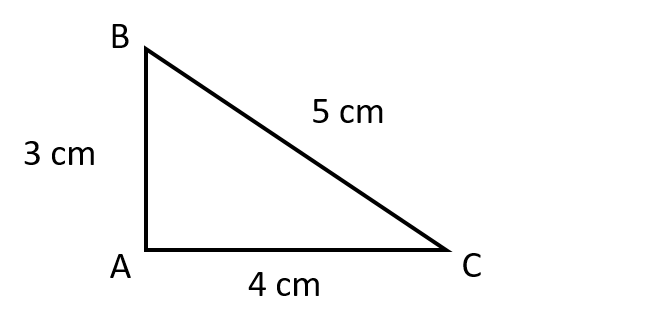
\includegraphics[scale=0.4]{Revision/Triangle_rectangle.png}
\end{figure}
\newpage
\textbf{2.} Le triangle ci-dessous est rectangle en A. Calculer la longueur AC :
\begin{figure}[!h]
    \centering
    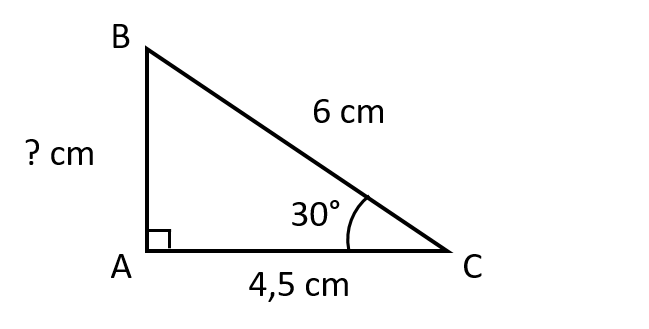
\includegraphics[scale=0.4]{Revision/Triangle_rectangle_2.png}
\end{figure}

\section{Physique}

\subsection{Record de vitesse ferroviaire}
Le projet de train japonais à sustentasion magnétique, le SCMaglev, a atteint la vitesse record de $603$~km/h en 2015. Ce train a la particularité de léviter au-dessus des rails. Pour rappel, un TGV roule à une vitesse de l'ordre de $300$~km/h en France.\\
\begin{enumerate}
    \item Convertir les deux vitesses en $m/s$.
    \item La distance entre Paris et Brest est de 500 km. En combien de temps une voiture roulant en moyenne à $100$~km/h effectue-t-elle ce trajet ? Et un TGV ? Et un SCMaglev ?
    \item Sachant que la distance Terre-Lune est de $380 000$~km, en combien de temps un SCMaglev peut-il atteindre la Lune ? On donnera la réponse en années/ jours/heures/minutes/secondes.
    \item A votre avis, quels sont les avantages du SCMaglev ?
\end{enumerate}

\subsection{Electricité}
\begin{enumerate}
    \item Avec quel instrument mesure-t-on une tension ? En quelle unité exprime-t-on le résultat ?
    \item Mêmes questions pour un courant.
    \item Une ampoule électrique est traversée par un courant I = $0,5$~A, et la tension à ses bornes est $U= 6$~V. Quelle est sa résistance ? Quelle puissance électrique $P$ consomme-t-elle ? 
    \item Faut-il utiliser un fil de cuivre ou un fil en caoutchouc pour conduire le courant ?
\end{enumerate}

\subsection{\'{E}nergie}
On rappelle qu’un corps de masse $m$ se déplaçant à la vitesse $v$ possède une énergie cinétique $E_c$ donnée par :
\begin{equation}
    E_c = \frac{1}{2}mv^2
\end{equation}
avec $E_c$ en J (Joule), $v$ en m/s et $m$ en kg.
\begin{enumerate}
    \item Une voiture pèse $m=1,2$ T. Convertir ce résultat en kg.
    \item Si cette voiture de masse roule à $50$~km/h, quelle est son énergie cinétique ?
    \item \textit{(bonus)} On branche pendant $\Delta t =1$~s une centrale nucléaire délivrant $1$~GW de puissance électrique à une voiture de masse $m=1000$~kg. \`{A} quelle vitesse va la voiture au bout de $\Delta t$ si on suppose que toutes l'énergie électrique fournit par la centrale a été convertie en énergie cinétique ?
\end{enumerate}

\section{Chimie}
\subsection{Atomes et petits pois}
\begin{enumerate}
    \item Quelle est la taille approximative d’un atome ? L’exprimer en m sous forme d’une puissance de 10.
    \item Combien d’atomes faut-il aligner pour obtenir une chaîne de longueur 1 mm ?
    \item Quels sont les principaux constituants d’un atome ?
    \item Modéliser physiquement un petit pois (forme, taille, ...). Si le noyau d’un atome avait la taille d’un petit pois, quelle taille aurait l’atome entier ?
\end{enumerate} 

\subsection{Verrerie}
\textbf{1.} Nommer la verrerie présentée ci-dessous :
\begin{figure}[!h]
    \centering
    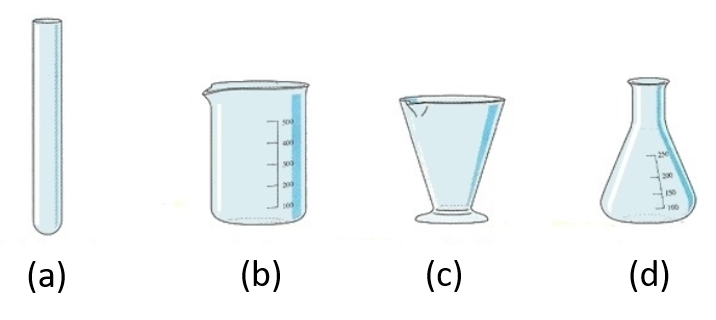
\includegraphics[scale=0.4]{Revision/Verrerie1.png}
\end{figure}

\textbf{2.} Proposer deux méthodes pour peser une masse $m=10$~g d'eau. On rappelle que la masse volumique de l'eau vaut $\rho=1$~g.mL${-1}$.
  %%\newpage
%$ $
%\newpage

\renewcommand{\thesubsection}{\textcolor{red}{\Roman{section}.\arabic{subsection}}}
\renewcommand{\thesubsubsection}{\textcolor{red}{\Roman{section}.\arabic{subsection}.\alph{subsubsection}}}

\setcounter{section}{0}
\sndEnTeteTPO

\begin{center}
\begin{mdframed}[style=titr, leftmargin=60pt, rightmargin=60pt, innertopmargin=7pt, innerbottommargin=7pt, innerrightmargin=8pt, innerleftmargin=8pt]

\begin{center}
\large{\textbf{TP 0: Des mesures en tout sens}}
\end{center}

\end{mdframed}
\end{center}



\begin{tcolorbox}[colback=blue!5!white,colframe=blue!75!black,title=Objectifs de la séance :]
\begin{itemize}
    \item S'approprier du matériel de mesure
    \item Appréhender les incertitudes d'une mesure
    \item Travailler en groupe
\end{itemize}
\end{tcolorbox}

Pour cette première séance de TP de l'année, nous allons manipuler quelques outils de mesures pour comprendre les sources d'incertitudes associées à ces mesures.

\section{Mesure du temps}
\begin{mdframed}[style=autreexo]
\textbf{\bsc{Liste du matériel}}
\begin{itemize}
    \item un pendule pesant
    \item un chronomètre
\end{itemize}
\end{mdframed}
\begin{Large}{\textbf{Q :}} \end{Large} La période d'oscillation d'un pendule est définie comme le temps au bout duquel le pendule a fait un aller-retour. Selon vous, comment peut-on mesurer le plus précisément la période d'oscillation du pendule ? \\
\newline
\newline
\underline{$1^{\text{ère}}$ méthode :} Lâcher le pendule d'une faible hauteur. Chaque élève mesure une période d'oscillation. \textbf{Comparer vos mesures entre vous et Commenter }:
\vspace{8cm}

\underline{$2^{\text{ème}}$ méthode :} Chaque binôme mesure 5 fois une période de manière indépendante. Notez les valeurs obtenues par binôme dans le tableau suivant :
\\

\begin{tabular}{|l|C{0.14}|C{0.14}|C{0.14}|C{0.14}|C{0.14}|C{0.14}|C{0.14}|C{0.14}|C{0.14}|C{0.14}|}
\hline
     Mesure n$^{\circ}$ & 1 & 2 & 3 & 4 & 5 \\
     \hline
     Période (en s) & & & & & \\
     \hline
\end{tabular}
\newline
\newline

\begin{tcolorbox}[colback=blue!5!white,colframe=white!75!black,title=Document 1 :]
La moyenne d'une mesure est la somme de toutes les valeurs mesurées divisée par le nombre de mesures effectuées :
\begin{equation*}
    \text{Moyenne} = \frac{\text{Mesure n$^{\circ}$1}+\text{Mesure n$^{\circ}$2} + ... + \text{Mesure n$^{\circ}$N}}{\text{N}}
\end{equation*}
L'écart-type représente la dispersion (c'est-à-dire à quel point les mesures changent d'une mesure à une autre) associée à une série d'une mesure. Elle est donnée par :
\begin{equation*}
    \text{Ecart-type }= \sqrt{\frac{\left(\text{Mesure n$^{\circ}$1}-\text{Moyenne}\right)^2+...+\left(\text{Mesure n$^{\circ}$N}-\text{Moyenne}\right)^2}{\text{N}}}
\end{equation*}
\end{tcolorbox}

\begin{tcolorbox}[colback=blue!5!white,colframe=white!75!black,title=Document 2 :]
On représente le résultat d'une mesure selon la manière suivante :
\begin{equation*}
    \text{Résultat} = \text{Moyenne} \pm \text{incertitude-type}
\end{equation*}
\end{tcolorbox}
\textbf{Travail à faire :} Calculer la moyenne notée $<T>$ de la période d'oscillation du pendule et évaluer qualitativement son incertitude-type. \underline{Pour les plus rapides :} calculer l'écart-type de vos mesures.

\newpage

\section{Mesure de la masse d'une bille de plomb}

\begin{mdframed}[style=autreexo]
\textbf{\bsc{Liste du matériel}}
\begin{itemize}
    \item 1 pied à coulisse
    \item 1 règle
    \item 1 balance
\end{itemize}
\end{mdframed}

\begin{tcolorbox}[colback=blue!5!white,colframe=white!75!black,title=Document 3 :]La masse $m$ d'une bille de plomb est reliée à son rayon $R$ et à sa masse volumique $\rho$ par la formule suivante :
\begin{equation*}
    m = \frac{4\pi R^3\times\rho}{3}
\end{equation*}
\end{tcolorbox}

\begin{Large}{\textbf{Q :}} \end{Large} Choisissez une bille de plomb, comment mesurer sa masse ? On donne $\rho=$
\newline
\newline

\underline{$1^{\text{ère}}$ méthode :} Mesurer la masse à la balance. \textbf{Commenter :}
\vspace{5cm}

\underline{$1^{\text{ère}}$ méthode :} Mesurer le rayon de la bille. En déduire la masse à l'aide du Document 3. \textbf{Commenter :}


\newpage

\section*{Conclusion du TP}

\begin{tcolorbox}[colback=red!5!white,colframe=red!75!black,title=\textbf{On retiendra : }]
\begin{enumerate}
    \item L'instrument de mesure et le protocole expérimental influent sur le résultat d'une mesure,
    \item On écrit un résultat expérimental final en prenant en compte son incertitude :
    \begin{equation*}
        \text{Résultat} = \text{Moyenne} \pm \text{incertitude-type}
    \end{equation*}
    \item On peut améliorer la mesure d'une grandeur physique en la répétant plusieurs fois et en calculant sa moyenne,
    \item On écrit un résultat en adaptant le nombre de chiffres significatifs.
\end{enumerate}
\end{tcolorbox}


%% Devoir Commun de seconde
  %\modeCorrection

%%%% Définition En-tête et pied de page 
\pagestyle{fancy}
\renewcommand\footrulewidth{1pt}
\fancyhead[L]{Devoir commun de Physique-Chimie}
\fancyhead[R]{Lycée Parc de Vilgénis}
\fancyfoot[C]{\textbf{Page \thepage/\pageref{LastPage}}}

\renewcommand{\thesubsection}{\textcolor{red}{\Roman{section}.\arabic{subsection}}}
\renewcommand{\thesubsubsection}{\textcolor{red}{\Roman{section}.\arabic{subsection}.\alph{subsubsection}}}
\renewcommand{\titreDocu}[1]{
  \refstepcounter{document} % update counter
  \textbf{Exercice \arabic{document} -- #1} 
  \addcontentsline{toc}{document}{\protect\numberline{} #1} % update table of content
}


\renewcommand{\numeroQuestion}{
  \refstepcounter{exercice}
  \vspace*{2pt}
  \hspace{15pt}
  \textcolor{black}{%couleurPrincipale!75!black}{
    \textbf{Q.\arabic{exercice}}
  }
}

\setcounter{section}{0}
\setcounter{document}{0}


%\nomPrenomClasse
\vspace{1cm}

\begin{center}
\begin{Huge}
    DEVOIR COMMUN DE SECONDE
\end{Huge}
\end{center}
\vspace{1cm}

\vspace{1cm}

\begin{center}
    \begin{large}
        Jeudi 21 Décembre 2023
    \end{large}
\end{center}

\vspace{2cm}

\begin{center}
    \begin{Large}
        \textbf{PHYSIQUE-CHIMIE}\\
    \end{Large}
\end{center}
\vspace{2cm}


\begin{center}
    \begin{large}
        Durée de l'épreuve : \textbf{2 heures}\\
    \end{large}
\end{center}
\vspace{1cm}
\begin{center}
    \begin{large}
        \textit{L'usage de la calculatrice est autorisé.}\\
    \end{large}
\end{center}
\vspace{1cm}
\begin{center}
    \begin{large}
        Dès que ce sujet vous est remis, assurez-vous qu’il est complet.\\
        Ce sujet comporte \pageref{LastPage} pages numérotées de \thepage/\pageref{LastPage} à \pageref{LastPage}/\pageref{LastPage}.
    \end{large}
\end{center}

\begin{tcolorbox}[colback=red!5!white,colframe=red!75!black,title=\textbf{Consignes : }]
   \begin{enumerate}
       \item Pour les élèves bénéficiant d'un tiers-temps, vous ne traiterez pas les questions marquées par $(*)$ ; 
       \item Lisez-bien l'énoncé des exercices. Les questions sont pour la plupart indépendantes. Si vous bloquez sur une question, passez à la suivante ;
       \item N'oubliez pas d'encadrer ou de souligner vos résultats ;
       \item Vous rendrez l'énoncé avec la copie.
   \end{enumerate}
\end{tcolorbox}
\newpage

%\begin{tableauCompetences}
%    APP & S'approprier les informations d'un document & & & & \\
%    \hline
%    REA & Utiliser les pourcentages et les fractions  & & & & \\
%     \hline 
%    ANA &  Exploiter les informations extraites des données & & & & \\
%    \hline
%    VAL & Valider/critiquer un modèle & & & &
%\end{tableauCompetences}



\begin{doc}{Le gaz de ville \begin{large}
    /9 points
\end{large}}
\vspace{-0.4cm}
\begin{wrapfigure}{r}{0.35\textwidth}
\vspace{-0cm}
    \centering
      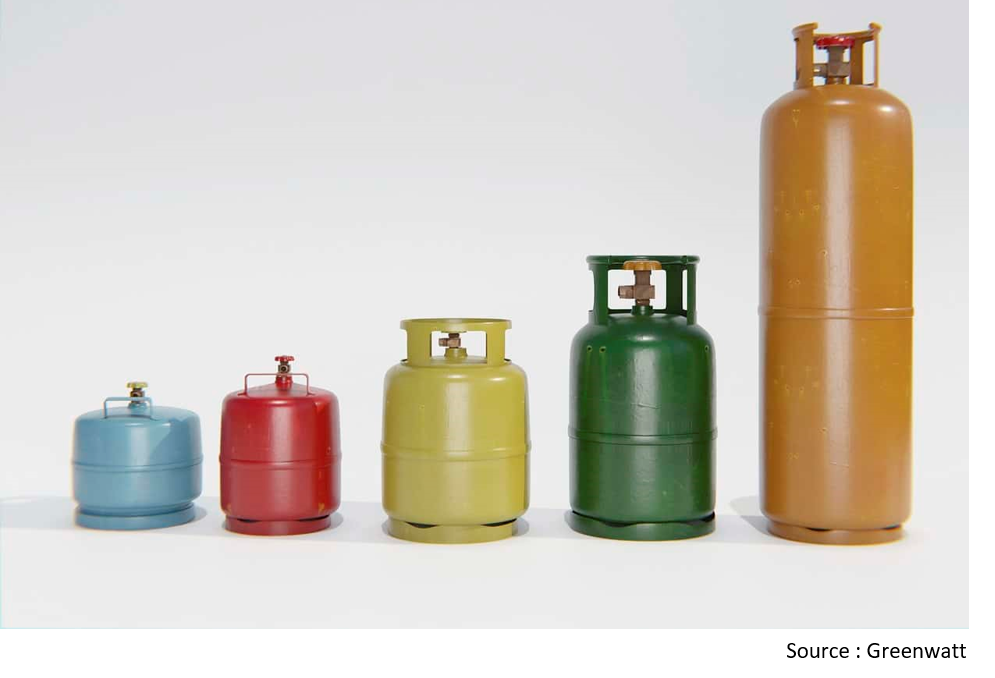
\includegraphics[scale=0.35]{Images/DS/Devoir_Commun/Bouteille_gaz.png}
  \end{wrapfigure}
L'odeur de gaz vous est désagréable, mais c'est pour votre bien ! Le saviez-vous ?\\
Le gaz de ville, celui qui arrive dans les habitations par des tuyaux de distribution collective, est principalement constitué de méthane. Le méthane est incolore et inodore, mais alors d'où vient l'odeur si caractéristique du gaz de ville ?\\
Ce que l'on appelle « odeur de gaz » est en réalité dû à un additif ajouté, le tétrahydrothiophène (THT), pour rendre les fuites de gaz détectables et prévenir du danger qu’elles représentent. En effet, le méthane devient fortement explosif lorsqu'il atteint une certaine concentration dans l'air.\\

On considère une bouteille de gaz de ville de volume $V=100$~L. L’étiquette sur la bouteille indique le pourcentage volumique des deux espèces chimiques présentes dans ce mélange :

\begin{center}
    \begin{tabular}{|C{0.45}|C{0.45}|}
        \hline
        \multicolumn{2}{|c|}{\cellcolor{blue!25}Composition du mélange contenu dans la bouteille de gaz de ville} \\
        \hline
        \cellcolor{orange!25}Nom de la substance & \cellcolor{orange!25}Pourcentage volumique \\
        \hline
        tétrahydrothiophène (THT) & 0,10225 \% \\
        \hline 
         Méthane & 99,89775 \%  \\
         \hline
    \end{tabular}
\end{center}
Voici quelques données sur le méthane :
\begin{center}
    \begin{tabular}{|c|C{0.3}|}
        \hline
        \cellcolor{orange!25}Pictogrammes de sécurité du méthane &
            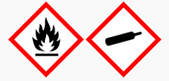
\includegraphics[scale=0.3]{Images/DS/Devoir_Commun/Picto.png}
         \\
        \hline
        \cellcolor{orange!25}Température de fusion (en $\degreCelsius$) à la pression atmosphérique & $-182,47$ \\
        \hline
        \cellcolor{orange!25}Température d'ébullition (en $\degreCelsius$) à la pression atmosphérique & $-161,52$ \\
        \hline 
        \cellcolor{orange!25}Masse volumique du méthane (en g$\cdot$L$^{-1}$) & 0,657 \\
         \hline
    \end{tabular}
\end{center}


\question{Rappeler la définition d’un mélange et proposer un exemple. (1pt)}{~}{0}
%\\
\vspace{-0.2cm}
\question{Il est conseillé de ne pas conserver une bouteille de méthane à proximité d’une fenêtre exposée au soleil. Justifier à l’aide des pictogrammes de sécurité du méthane.(1pt)
}{}{0}
%\\
\vspace{-0.2cm}
\question{Indiquer l’état physique du méthane à température ambiante (20°C) et à la pression atmosphérique. Justifier. (1pt)}{}{0}
%\\
\vspace{-0.2cm}
\question{\`{A} l’aide des documents, déterminer le volume de chaque espèce chimique présente dans la bouteille de gaz de ville. (2pts)}{~}{0}
\newpage%\\
\question{$(*)$ En déduire la masse de méthane $m_{\text{méthane}}$ contenue dans la bouteille. (1pt)}{~}{0}
%\\
Voici un graphe donnant la masse volumique du mélange méthane/THT en fonction du pourcentage volumique du THT dans le mélange : 
\begin{center}
    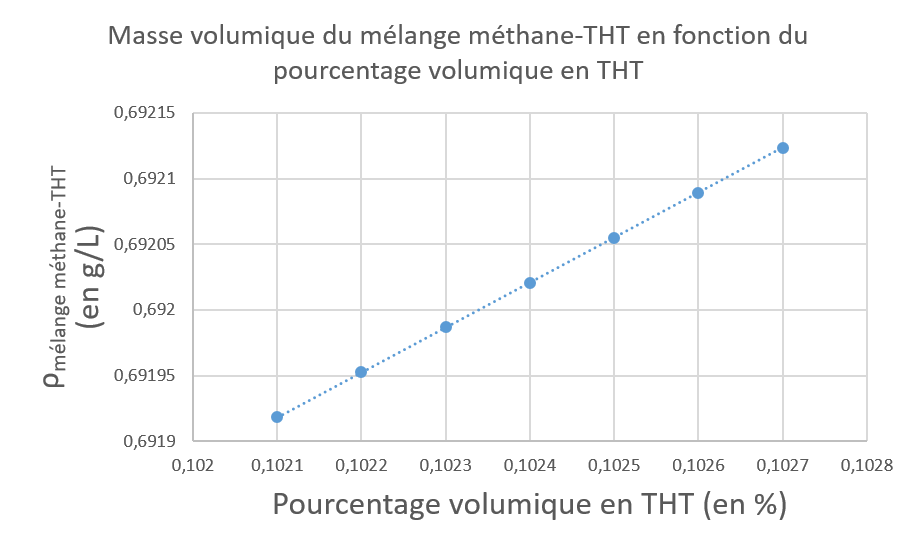
\includegraphics[scale=1]{Images/DS/Devoir_Commun/Graphe_rhovspourcentagevol.png}
\end{center}
\question{Déterminer graphiquement la masse volumique du mélange $\rho_{\text{mélange}}$ dans la bouteille de gaz de ville. Vous ferez apparaître la construction sur le graphique. (1pt)}{~}{0}
%\\
\textbf{Pour la question suivante, toute tentative de réponse même non aboutie sera valorisée.}\\
\question{$(*)$ La norme imposée au gaz de ville est qu’il doit contenir entre $15$~mg et $40$~mg de THT par litre de gaz. Exprimer la masse volumique du mélange en fonction de la masse des espèces chimiques et du volume de la bouteille. En déduire la masse de THT présente dans la bouteille de gaz étudiée. Respecte-t-elle la norme imposée au gaz de ville ? Justifier en rédigeant une réponse scientifiquement argumentée. (2pts)}{On trouve 36~mg.}{0}
%\\
\end{doc}

%%%%%%%%%%%%%%%%%%%%%%%%%%%%%%%%%
\newpage
%%%%%%%%%%%%%%%%%%%%%%%%%%%%%%%%%
\setcounter{exercice}{0}
\begin{doc}{Solutions aqueuses \begin{Large}
    /9 points
\end{Large}}
\begin{wrapfigure}{r}{0.3\textwidth}
\vspace{-1cm}
    \centering
      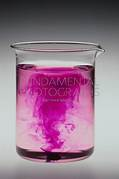
\includegraphics[scale=1.0]{Images/DS/Devoir_Commun/Permanganate.png}
  \end{wrapfigure}
\og Le permanganate de potassium est un solide gris-violet de formule \chemform{KMnO_4}. Dissous dans l’eau, il donne des solutions de couleur violette.\\
Pour soigner les érythèmes (irritations de la peau), il est recommandé d’utiliser des solutions aqueuses de permanganate de potassium de concentration en masse égale à $0,10$~g$\cdot$L$^{-1}$.\\
En solution aqueuse à $0,50$~g$\cdot$L$^{-1}$, le permanganate de potassium est également utilisé comme désinfectant pour laver les légumes dans les pays tropicaux.\fg
\begin{flushright}
    \textit{D’après le site \url{ societechimiquedefrance.fr/permanganate-de-potassium}}.
\end{flushright}

L’objectif de l’exercice est d’estimer la concentration d’une solution aqueuse S de permanganate de potassium afin de valider ou non son utilisation pour soigner les érythèmes ou pour laver les légumes.\\

Pour cela, on prépare 250 mL d’une solution aqueuse S$_0$ de permanganate de potassium de concentration en masse $C_{m,0} = 0,60$~g$\cdot$L$^{-1}$ en dissolvant dans l’eau une masse appropriée de permanganate de potassium solide.\\


\question{Identifier le solvant et le soluté des solutions utilisées pour soigner les érythèmes ou pour laver les légumes. (1pt)}{Solvant : eau, soluté : \chemform{KMnO_4}.}{0}
%\\
\question{$(*)$ Donner le nom de la technique utilisée pour préparer la solution S$_0$. (0,5pt)}{Il s'agit d'une dissolution.}{0}
%\\
\question{Donner l’expression de la concentration en masse $C_m$ d’une solution en fonction de la masse de soluté $m_{\text{soluté}}$ et du volume de solution $V_{\text{solution}}$. (0,5pt)}{}{0}
%\\
\question{En déduire la valeur de la masse de permanganate de potassium qui a été dissoute pour préparer 250 mL de solution S$_0$. (1,5pts)}{~}{0}
%\\

\newpage
On prépare ensuite cinq solutions S$_1$, S$_2$, S$_3$, S$_4$ et S$_5$ en prélevant différents volumes de solution aqueuse S$_0$ de permanganate de potassium de concentration en masse $C_{m,0} = 0,60$~g$\cdot$L$^{-1}$ et en y ajoutant de l’eau distillée pour obtenir un volume de 50,0 mL de solution (voir tableau ci-après).
\begin{center}
    \begin{tabular}{|C{0.1}|C{0.2}|C{0.2}|C{0.3}|}
        \hline
        \cellcolor{blue!25}Solution & \cellcolor{blue!25}Volume de solution S$_0$ à prélever (mL) & \cellcolor{blue!25}Volume de solution obtenue (mL) & \cellcolor{blue!25}Concentration en masse de la solution obtenue (g$\cdot$L$^{-1}$) \\
        \hline 
        S$_1$ & 2 & 50,0 & 0,024 \\
        \hline
        S$_2$ & 5 & 50,0 & 0,060 \\
        \hline
        S$_3$ & 10 & 50,0 & 0,12 \\
        \hline
        S$_4$ & 15 & 50,0 & 0,18 \\
        \hline
        S$_5$ & ~? & 50,0 & 0,24 \\
        \hline
    \end{tabular}
\end{center}

\question{Donner le nom de la technique utilisée pour préparer les cinq solutions S$_1$, S$_2$, S$_3$, S$_4$ et S$_5$. (0,5pt)}{Il s'agit d'une dilution.}{0}
%\\
\question{Écrire le protocole expérimental qui a été suivi pour préparer 50,0 mL de solution S$_1$. Préciser soigneusement le nom du matériel utilisé. (1,5pts)}{~}{0}
%\\
\question{Déterminer la valeur du volume de solution S$_0$ qui a été prélevé pour préparer 50,0 mL de solution S$_5$. Justifier précisément le calcul effectué. (2pts)}{~}{0}
%\\
On verse les cinq solutions S$_1$, S$_2$, S$_3$, S$_4$ et S$_5$ dans des tubes à essais : on obtient ainsi une échelle de teintes (voir photo ci-dessous).
\begin{center}
    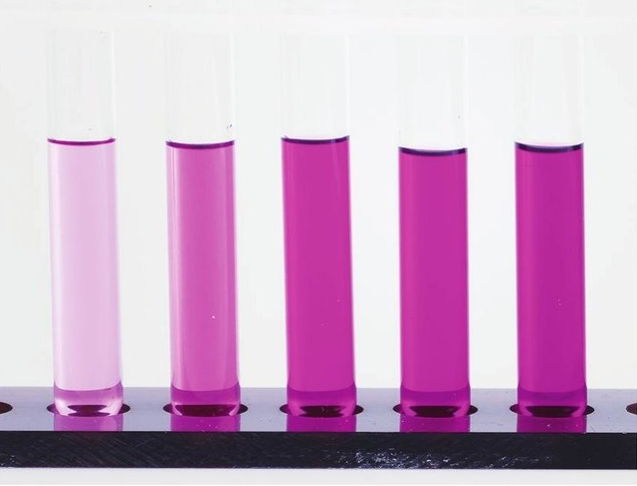
\includegraphics[scale=0.5]{Images/DS/Devoir_Commun/Echelle_teinte.png}
\end{center}
On verse ensuite la solution S dans un sixième tube à essais. On constate que la teinte de la solution S est comprise entre celles des solutions S$_2$ et S$_3$.\\
\question{Déterminer un encadrement de la concentration en masse de la solution S. (1pt)}{$0,060~\text{g$\cdot$L$^{-1}$}<C_{m,0}<0,12~\text{g$\cdot$L$^{-1}$}$}{0}
%\\
\question{$(*)$ En déduire si la solution $S$ peut être utilisée pour soigner les érythèmes ou pour laver les légumes. Justifier.(0,5pt)}{~}{0}
\end{doc}
\setcounter{exercice}{0}
\begin{doc}{Le son d’une guitare
 \begin{Large}
    /12 points
\end{Large}}
Une guitare se compose d'un coffre auquel est accroché un manche sur lequel sont tendues des cordes métalliques ou en nylon. La photo ci-dessous présente une guitare ainsi qu'un zoom sur une partie du manche après avoir frotté les cordes :

\begin{center}
    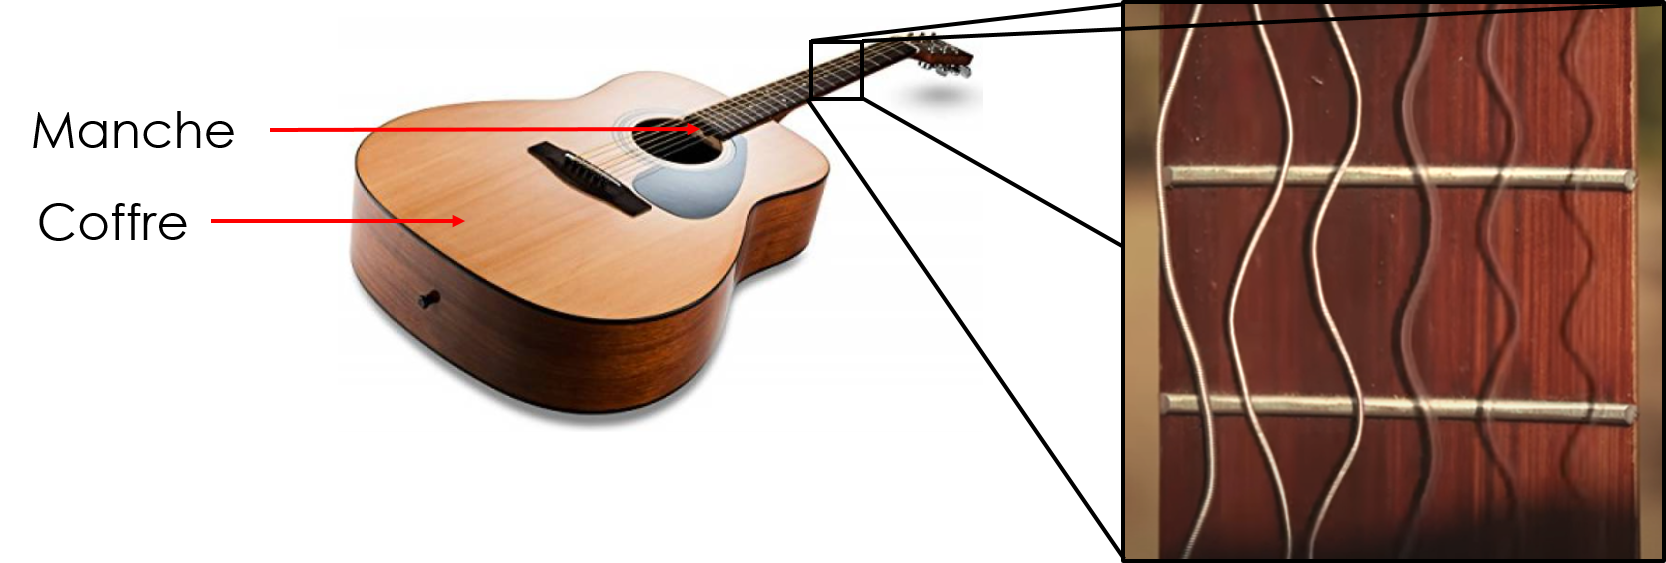
\includegraphics[scale=0.5]{Images/DS/Devoir_Commun/Guitare.png}
\end{center}

Voici un tableau des notes (do, ré, mi, fa, sol, la, si) et des fréquences (en Hz) correspondantes de la gamme tempérée :
\begin{center}
    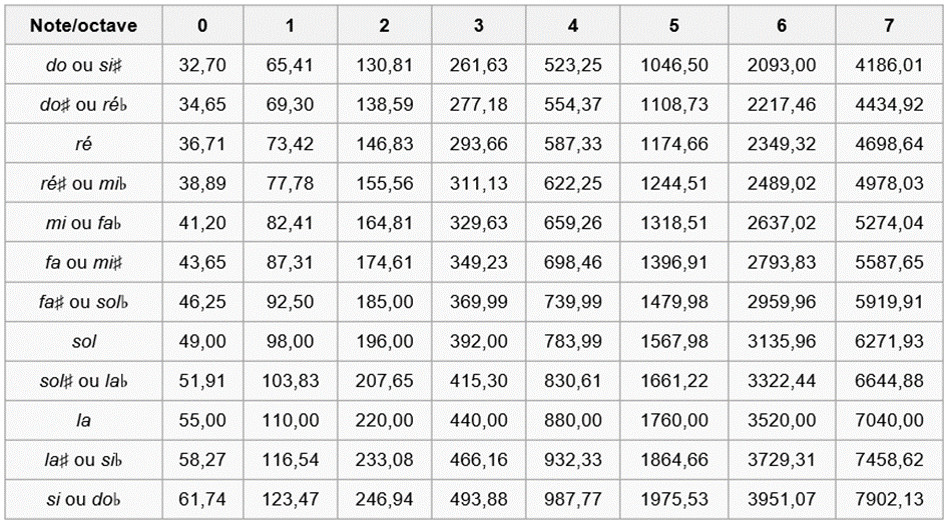
\includegraphics[scale=0.7]{Images/DS/Devoir_Commun/Notes_guitare.png}
\end{center}

On dit qu'une note est jouée \og à vide \fg~ lorsqu'on laisse la corde de guitare vibrer librement sur toute sa longueur. De la corde la plus épaisse à la plus fine, les six notes jouées à vide sont : \og mi2, la2, ré3, sol3, si3, mi4 \fg~.
\newpage
\question{Indiquer l'origine du son émis par une guitare. (1pt)}{Les cordes vibrent et font vibrer les molécules d'air de proche en proche.}{0}
%\\
\question{Donner l'intérêt physique du coffre d'une guitare. (1pt)}{Le coffre sert de caisse de résonance, c'est-à-dire qu'il sélectionne et amplifie et le son émis par le frottement des cordes de guitare.}{0}
%\\
\question{Indiquer la condition pour que le son se propage dans un milieu. (0,5pt)}{Il faut un milieu matériel pour que le son puisse se propager}{0}
%\\
\question{Identifier le milieu dans lequel le son se propage de la guitare jusqu'à notre oreille puis rappeler la valeur de la vitesse de propagation du son dans ce milieu. (1pt)}{Ici, le milieu est l'air et la vitesse vaut (à $15\degreCelsius$) 340~m$\cdot$s$^{-1}$.}{0}
%\\
\question{Calculer la durée $\Delta t$ que met le son à se propager jusqu’à l’auditeur lorsqu'il se trouve à une distance d=1km. (2pts). \textit{(Bonus) : l'auditeur parviendre-t'il a entendre ce son ? Justifier. (1pt)}}{~}{0}
%\\
\question{$(*)$ Donner le domaine des fréquences audibles pour un être humain. (1pt)}{Entre 20~Hz et 20000~Hz.}{0}
%\\
\question{Un chat est capable d’entendre des fréquences comprises entre 20 Hz et 60 kHz. Peut-il entendre la note la plus grave jouée avec une guitare ? Justifier la réponse. (1pt)}{Oui car la note la plus grave sonne à la fréquence 32,70~Hz qui est comprise dans le domaine de fréquence audible du chat.}{0}
%\\
\question{$(*)$ Donner les valeurs des fréquences des 6 notes jouées à vides à la guitare. (1,5pts)}{~}{0}
%\\
\question{Entre la note mi2 et la note mi3, donner le son le plus aigu. Justifier.(1pt)}{~}{0}
%\\
Un ingénieur du son a enregistré une note émise par une guitare, à l’aide d’un microphone relié à un système informatisé. Voici le signal enregistré :
\begin{center}
    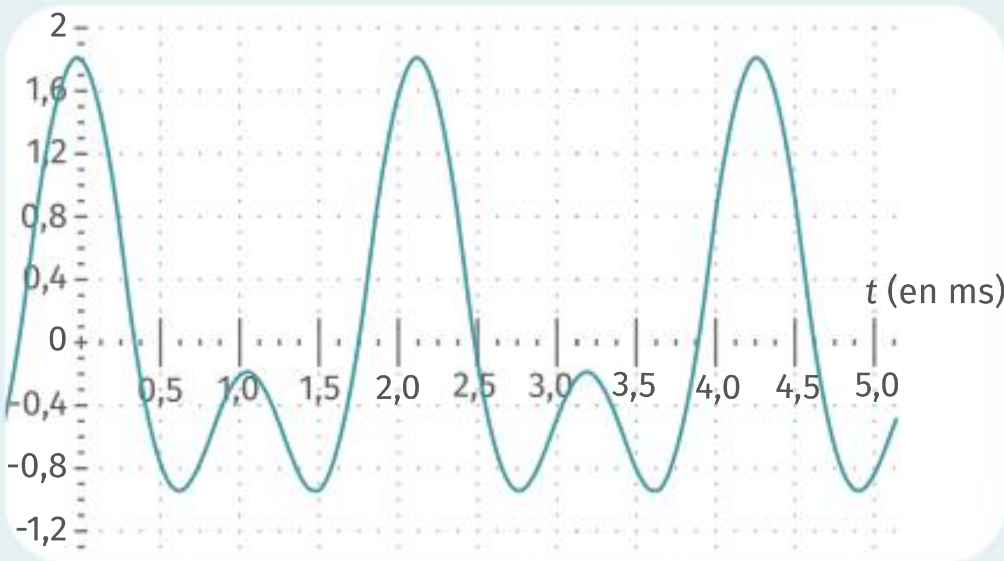
\includegraphics[scale=0.5]{Images/DS/Devoir_Commun/Signal_guitare.PNG}
\end{center}
\question{Donner la formule reliant la fréquence $f$ et la période $T$ d’un signal. Déterminer la fréquence $f$ de la note émise par la guitare. (2pts)}{~}{0}

\end{doc}
\vspace{2cm}
\begin{center}
\begin{Huge}
    \textbf{FIN DU SUJET.}
\end{Huge}
\end{center}
  
%%%%%%%%%%%%%%% Methodo %%%%%%%%%%%%%%%%%%%%%
  %\newpage

\renewcommand{\thesubsection}{\textcolor{red}{\Roman{section}.\arabic{subsection}}}
\renewcommand{\thesubsubsection}{\textcolor{red}{\Roman{section}.\arabic{subsection}.\alph{subsubsection}}}

\setcounter{section}{0}
\sndEnTeteMethodoUn

\begin{center}
\begin{mdframed}[style=titr, leftmargin=60pt, rightmargin=60pt, innertopmargin=7pt, innerbottommargin=7pt, innerrightmargin=8pt, innerleftmargin=8pt]

\begin{center}
\large{\textbf{Fiche méthode 1 : Outils pour la Physique et la Chimie}}
\end{center}

\end{mdframed}
\end{center}
Ce chapitre présente quelques rappels sur les outils mathématiques, les méthodes et les représentations que nous utiliserons toute l'année en physique comme en chimie. Il est donc essetiel de maîtriser ces notions pour démarrer l'année sur d'excellentes bases. N'hésitez pas à le reconsulter toute l'année au besoin !

\begin{tcolorbox}[colback=blue!5!white,colframe=blue!75!black,title=Mots clés du chapitre :]
Puissance de $10$, unités SI, règles de sécurité en chimie
\end{tcolorbox}

\section{Puissance de 10}
\subsection{Représentation}
Les nombres très grands ou très petits s'écrivent à l'aide des puissances de 10 :
\begin{align*}
    10^n &= \underbrace{10\times10\times ... \times 10}_{\text{\textbf{n} "10 $\times$"}} = 1\underbrace{00...0}_{\text{\textbf{n} zéros}} \\
    10^{-n} &= \frac{1}{10^n} = 0,0....0\underbrace{1}_{\text{en \textbf{n-ième} position}}
\end{align*}

\underline{Exemples :} $10^9$ = 1 000 000 000,    $10^{-5}$=0,000 01\\

\subsection{Opérations}
\begin{tcolorbox}[colback=red!5!white,colframe=red!75!black,title=\textbf{Règles de calculs des puissances de 10}]
Soit $a$ et $b$ deux nombres réels.
\begin{align*}
    10^{a}\times 10^b &= 10^{a+b} & \text{Ex :}& 10^{1}\times 10^2 = 10^{1+2}=10^3 \\
    \frac{10^{a}}{10^b} &= 10^{a-b} & \text{Ex :}& \frac{10^{1}}{10^2} = 10^{1-2}=10^{-1} \\
\end{align*}

\end{tcolorbox}
\underline{Effectuer les calculs suivants :}
\begin{align*}
    10^{30} \times 10^{50} &= 10^{30+50}=10^{80} & \frac{10^{2033}}{10^{10}} &= 10^{2033-10} = 10^{2023} & \frac{10^2}{10^8}\times 10^5 &= 10^{2-8+5} = 10^{-1}
\end{align*}
\subsection{Notation scientifique}

\begin{tcolorbox}[colback=green!5!white,colframe=green!75!black,title=\textbf{Ecriture scientifique d'un nombre}]
En écriture scientifique, une valeur numérique s'exprime sous la forme :
\begin{equation*}
    a \times 10^n
\end{equation*}
avec $n$ un nombre entier relatif et $a$ un nombre décimal tel que : $1< a <10$.\\
\\
\end{tcolorbox}
\underline{Exemples :}
\begin{itemize}
    \item la masse $M_{L}$ de la Lune vaut $M_{Lune}=734$ $800$ $000$ $000$ $000$ $000$ $000$~kg et s'écrit donc plus simplement : $M_L=7,348\times 10^{20}$~kg
    \item La taille $d$ d'une molécule d'eau est de  $d=0,000$ $000$ $003$ $4$~m, soit en écriture scientifique : $d=3,4\times10^{-9}$~m
\end{itemize}

\subsection{Ordre de grandeur}
\begin{tcolorbox}
[colback=green!5!white,colframe=green!75!black,title=\textbf{Ordre de grandeur d'un nombre}]
L'ordre de grandeur d'un nombre et la puissance de 10 la plus proche de ce nombre.
\end{tcolorbox}
\underline{Exemples :}
\begin{itemize}
    \item Ordre de grandeur de 30 000 = 10$^4$
    \item Ordre de grandeur de 0,000 007 = 10$^{-5}$
    \item Ordre de grandeur de 8 700 000 = 10$^6$
    \item Ordre de grandeur de 0,000 256 = 10$^{-4}$
\end{itemize}

\section{Unités}
\subsection{Les unités du système international SI}
Depuis 2019, la communauté scientifique internationale, à travers la "Conférence générale des poids et mesures", a adopté un système d'unités universel. Leur valeur sont définies à partir de 7 constantes universelles dont les valeurs exactes ont été définitivement "fixées" en Novembre 2018 (\textit{source Wikipédia}). 
\begin{figure}[!h]
    \centering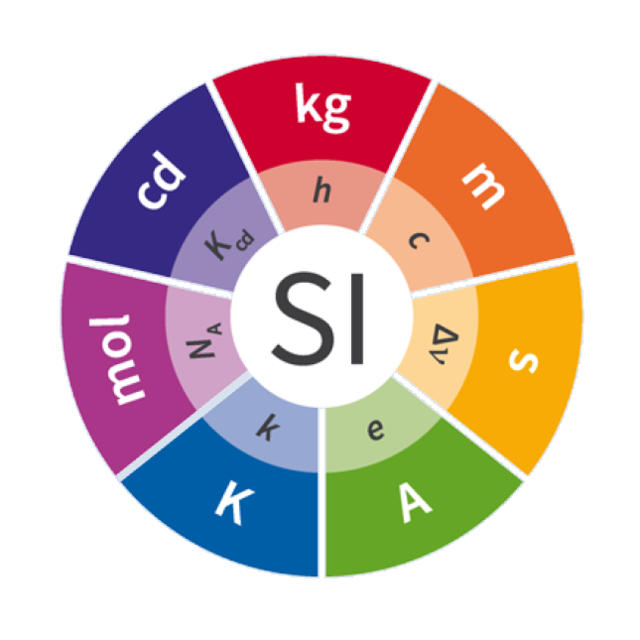
\includegraphics[scale=0.4]{Images/Methodo/Fiche_Methode1/SI_Logo_with_defining_constants.png}
    \caption{Logo du système SI. }
    \label{fig:Syteme_SI}
\end{figure}
\begin{table}[!h]
    \centering
    \begin{tabularx}{\textwidth}{| X | X | c | X |}  \hline
Grandeur physique & Unité SI & Symbole de l'unité & Appareil de mesure \\
\hline
Masse & kilogramme & kg & balance \\
Temps & seconde & s & chronomètre \\
Longueur & mètre & m & règle \\
Température & kelvin & K & thermomètre \\
Intensité électrique & ampère & A & ampèremètre \\
Quantité de matière & mole & mol & balance\\
Intensité lumineuse & candela & cd & luxmètre \\
\hline
\end{tabularx}
    \caption{Tableau des unités du SI et les appareils de mesure associés.}
    \label{tab:SI}
\end{table}
\importantbox{Nous utilisons courament d'autres unités qui nous paraissent bien plus pratiques dans leur utilisation. Par exemple, nous utilisons plus facilement les degrés celsius $^\circ$C pour la température ou encore les tailles XS, S, M, L, ... pour les vêtements (même si la relation entre ces dernières \og unités \fg et les unités du SI semble très obscure...).}


\subsection{Préfixes des unités.}
Il est très souvent utile et agréable de remplacer l’écriture scientifique d’un nombre par \textbf{un nombre écrit sans puissance de 10 suivi d'un multiple ou sous-multiple de l'unité du nombre}.
\begin{table}[!h]
    \centering
    \begin{tabular}{|C{0.15}|c|c|}
    \hline
    Multiple ou sous-multiple & Facteur par lequel l'unité est multipliée & Exemple typique \\ 
    \hline 
    Multiple & 1 000 000 000 000 = $10^{12}$ & Téraoctet (To) \\
    \hline
    Multiple & 1 000 000 000 = $10^{9}$ & Gigaoctet (Go)\\
    \hline
    Multiple & 1 000 000 = $10^{6}$ & Mégajoule (MJ)\\
    \hline
    Multiple & 1 000 = $10^{3}$ & kilogramme (kg)\\
    \hline
    Multiple & 100 = $10^{2}$ & hectomètre (hm)\\
    \hline
    Multiple & 10 = $10^{1}$ &  decalitre (daL)\\
    \hline
    Sous-Multiple & 0,1 = $10^{-1}$ & decimètre (dm) \\
    \hline
    Sous-Multiple & 0, 01 = $10^{-2}$ & centilitre (cL) \\
    \hline
    Sous-Multiple & 0, 001 = $10^{-3}$ & milliseconde (ms) \\
    
    \hline
    Sous-Multiple & 0, 000 001 = $10^{-6}$ & micromètre ($\mu$m)\\
    \hline
    Sous-Multiple & 0, 000 000 001 = $10^{-9}$ & nanoseconde (ns) \\
    \hline
    Sous-Multiple & 0, 000 000 000 001 = $10^{-12}$ & picomètre (pm)\\
    \hline
    Sous-Multiple & 0, 000 000 000 000 001 = $10^{-15}$ & femtomètre (fm)\\
    \hline
    \end{tabular}
    
    \caption{Tableaux des préfixes des multiples et sous multiples}
    \label{tab:chap1_multiples}
\end{table}

\section{Chiffres significatifs}

\begin{tcolorbox}
[colback=green!5!white,colframe=green!75!black,title=\textbf{Chiffre significatif}]
Lorsqu’on écrit une valeur en notation scientifique, le nombre de chiffres employés dans le facteur avant la puissance de 10 est le nombre de chiffres significatifs.\\
\end{tcolorbox}
Exemples : 
\begin{itemize}
    \item la célérité de la lumière $c$ dans le vide est :
\begin{equation*}
    c =\underbrace{2,99 792458}_{\text{9 chiffres significatifs}}\times 10^8~\text{m.s}^{-1}
\end{equation*}
\item 0,002 3 possède 2 chiffres significatifs car il s'écrit : $2,3\times10^{-3}$ en notation scientifique.
\end{itemize}

\begin{tcolorbox}[colback=red!5!white,colframe=red!75!black,title=Règles à retenir sur les chiffres significatifs]
Le résultat d'une somme, différence, produit ou quotient est écrit avec \textbf{le plus petit nombre de chiffres signifcatifs présents dans les grandeurs dans son calcul}.
\newline
\newline
\textit{Exemple : } Calculer le temps $\Delta t$ pour que la lumière parcourt la distance Terre-Soleil $d=150\times 10^{6}$~km. Attention à mettre les grandeurs dans les bonnes unités.
\end{tcolorbox}


\section{Rédaction d'un calcul}
La réponse à une question demandant un calcul ne se résume pas l'invocation simple d'une formule non commentée et un résultat sans unité (à part bien sûr si le résultat attendu est sans unité). A chaque étape, on doit répondre de manière argumentée et présentable un calcul. Prenons l'exemple suivant : 

\begin{mdframed}[style=autreexo]
\textbf{\bsc{Exercice} - Distance Paris-Brest en train}\\
 Un TGV roule à une vitesse de l'ordre de $3,0\times 10^{2}$~km/h en France. La distance entre Paris et Brest est de 580 km.
\begin{enumerate}
\item En combien de temps une voiture roulant en moyenne à $100$~km/h effectue-t-elle ce trajet ?
\item Et un TGV ?
\end{enumerate}
\end{mdframed}

\begin{minipage}{0.5\textwidth}
    \begin{tcolorbox}[colback=red!5!white,colframe=red!75!black,title=\textbf{Mauvaise rédaction : }]
    \textbf{1)} 5,80 \\
    \textbf{2)} 1,93333333\\
    \end{tcolorbox}
\end{minipage}
\begin{minipage}{0.5\textwidth}
    \begin{tcolorbox}[colback=green!5!white,colframe=green!75!black,title=\textbf{Bonne rédaction : }]
    \textbf{1)} Le temps de parcours est donné par la formule $\Delta t=\frac{d}{v}$ avec $d$ la distance Paris-Brest et $v$ la vitesse de la voiture. Avec les données de l'énoncé, on obtient un temps de parcourt pour la voiture de :
    \begin{equation*}
        \Delta t = \frac{580}{100} = 5,8~\text{h}
    \end{equation*}
    \textbf{2)} En utilisant la même formule que la question précédente, on obtient un temps de parcourt pour le TGV de :
     \begin{equation*}
        \Delta t = \frac{580}{3,0\times 10^2} = 1,9~\text{h}
    \end{equation*}
    \end{tcolorbox}
\end{minipage}


\section{Règles de sécurité en TP de chimie}
\subsection{Les règles de sécurité}
\begin{tcolorbox}[colback=red!5!white,colframe=red!75!black,title=\textbf{En TP de chimie :}]
\begin{itemize}
    \item Je porte les EPI (Equipements de Protection Individuel) le cas échéant ;
    \item On ne jette pas les produits chimiques dans le lavabo sauf contre-indication ;
    \item On ne respire pas, ne mange pas et ne boit pas un produit chimique (même si comestible !) ;
    \item On fait attention/respecte le matériel ;
    \item On vérifie les pictogrammes de sécurité lorsqu'on manipule un produit chimique ;
    \item On range et nettoie son plan de travail à la fin du TP ;
\end{itemize}
\end{tcolorbox}

\subsection{Les pictogrammes de sécurité et EPI}
\begin{figure}[!h]
    \centering
    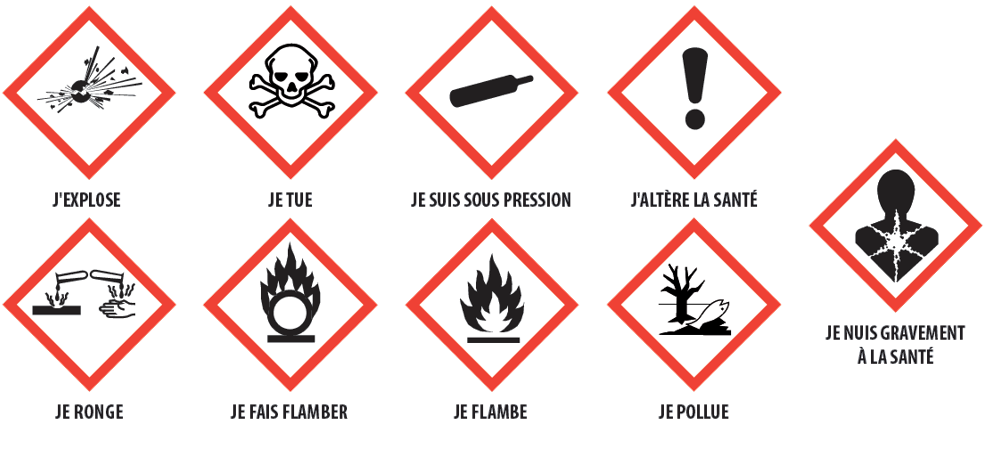
\includegraphics[scale=1]{Images/Methodo/Fiche_Methode1/Pictogrammes.png}
    \caption{Pictogrammes de sécurité}
    \label{fig:enter-label}
\end{figure}

\begin{figure}[!h]
    \centering
    
\includegraphics[scale=0.9]{Images/Methodo/Fiche_Methode1/picto_gant_blouse_lunette.jpg}
    \caption{Logo des \'{E}quipements de Protection Individuelle (EPI)}
    \label{fig:enter-label}
\end{figure}

\importantbox{Si vous avez un doute concernant un produit non étiquetté, il ne faut pas hésiter à regarder sa fiche de données de sécurité sur le site de l'INRS (Institut National de Recherche et de Sécurité) : \url{https://www.inrs.fr/publications/bdd/fichetox.html}}

\underline{\textbf{Exemple :}}
\begin{figure}[!h]
    \centering
    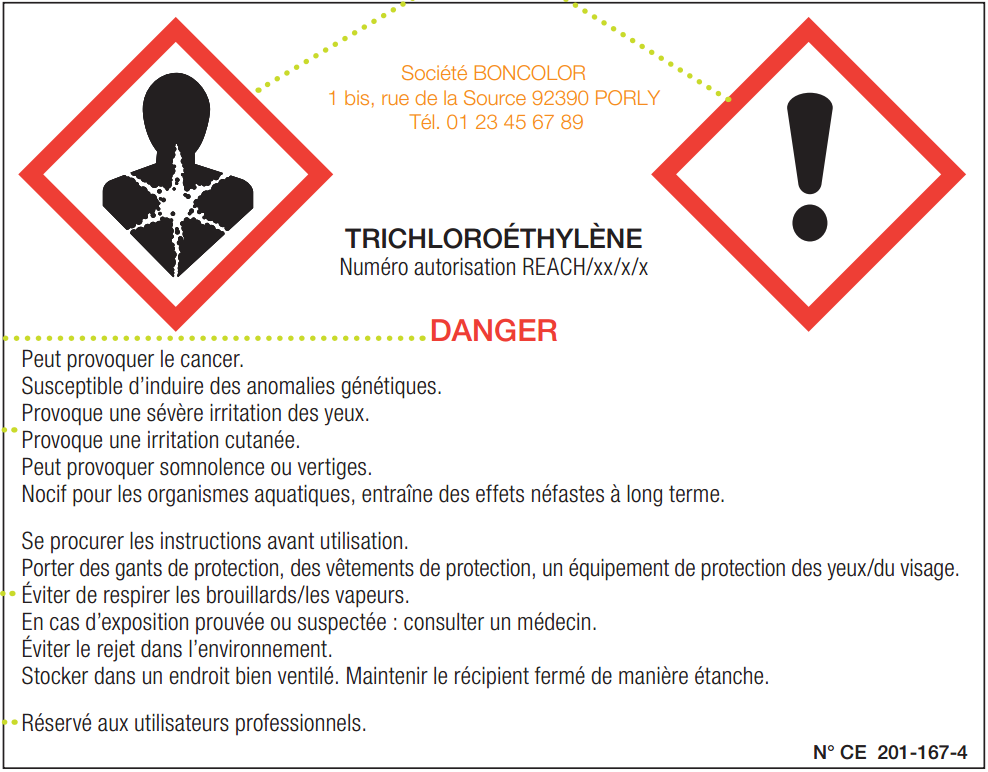
\includegraphics[scale=0.7]{Images/Methodo/Fiche_Methode1/Exemple_fiche_toxico.PNG}
    \caption{Exemple d'une fiche de données de sécurité sur)àoi le site de l'INRS.}
    \label{fig:enter-label}
\end{figure}



%%%%%%%%%%%%%%%%%%%%%%%%%%%%%%%%%%%%%%%%%%%%%
\end{document}